\documentclass[12pt]{article}\usepackage[]{graphicx}\usepackage[]{color}
%% maxwidth is the original width if it is less than linewidth
%% otherwise use linewidth (to make sure the graphics do not exceed the margin)
\makeatletter
\def\maxwidth{ %
  \ifdim\Gin@nat@width>\linewidth
    \linewidth
  \else
    \Gin@nat@width
  \fi
}
\makeatother

\definecolor{fgcolor}{rgb}{0.345, 0.345, 0.345}
\newcommand{\hlnum}[1]{\textcolor[rgb]{0.686,0.059,0.569}{#1}}%
\newcommand{\hlstr}[1]{\textcolor[rgb]{0.192,0.494,0.8}{#1}}%
\newcommand{\hlcom}[1]{\textcolor[rgb]{0.678,0.584,0.686}{\textit{#1}}}%
\newcommand{\hlopt}[1]{\textcolor[rgb]{0,0,0}{#1}}%
\newcommand{\hlstd}[1]{\textcolor[rgb]{0.345,0.345,0.345}{#1}}%
\newcommand{\hlkwa}[1]{\textcolor[rgb]{0.161,0.373,0.58}{\textbf{#1}}}%
\newcommand{\hlkwb}[1]{\textcolor[rgb]{0.69,0.353,0.396}{#1}}%
\newcommand{\hlkwc}[1]{\textcolor[rgb]{0.333,0.667,0.333}{#1}}%
\newcommand{\hlkwd}[1]{\textcolor[rgb]{0.737,0.353,0.396}{\textbf{#1}}}%

\usepackage{framed}
\makeatletter
\newenvironment{kframe}{%
 \def\at@end@of@kframe{}%
 \ifinner\ifhmode%
  \def\at@end@of@kframe{\end{minipage}}%
  \begin{minipage}{\columnwidth}%
 \fi\fi%
 \def\FrameCommand##1{\hskip\@totalleftmargin \hskip-\fboxsep
 \colorbox{shadecolor}{##1}\hskip-\fboxsep
     % There is no \\@totalrightmargin, so:
     \hskip-\linewidth \hskip-\@totalleftmargin \hskip\columnwidth}%
 \MakeFramed {\advance\hsize-\width
   \@totalleftmargin\z@ \linewidth\hsize
   \@setminipage}}%
 {\par\unskip\endMakeFramed%
 \at@end@of@kframe}
\makeatother

\definecolor{shadecolor}{rgb}{.97, .97, .97}
\definecolor{messagecolor}{rgb}{0, 0, 0}
\definecolor{warningcolor}{rgb}{1, 0, 1}
\definecolor{errorcolor}{rgb}{1, 0, 0}
\newenvironment{knitrout}{}{} % an empty environment to be redefined in TeX

\usepackage{alltt}
\usepackage{amsmath}
\usepackage{amssymb}
\usepackage{graphicx}
\usepackage{fullpage}
\usepackage{setspace}
\usepackage{hyperref}
\usepackage{color}
\onehalfspacing
\IfFileExists{upquote.sty}{\usepackage{upquote}}{}
\begin{document}

\title{Pol Sci 630: Problem Set 13 - Autocorrelation, Fixed, Random, Mixed Effects, and Causal Inference Techniques - Solutions}

\author{Prepared by: Jan Vogler (\href{mailto:jan.vogler@duke.edu}{jan.vogler@duke.edu})}

\date{Grading Due Date: Friday, December 4th, 12.00 PM}
 
\maketitle



\textbf{\color{red} Insert your comments on the assignment that you are grading above the solution in bold and red text. For example write: "GRADER COMMENT: everything is correct! - 4/4 Points" Also briefly point out which, if any, problems were not solved correctly and what the mistake was.}

\bigskip

\textbf{Use the following scheme to assign points: For problems that were solved correctly in their entirety, assign the full point value of 4. For correctly solved bonus problems, add that value to the total score for a problem but do not go above 4 points per problem. If there are mistakes in any problem, subtract points according to the extent of the mistake. If you subtract points, explain why.}

\bigskip

\textbf{In order to make your text bold and red, you need to insert the following line at the beginning of the document:}

\begin{verbatim} \usepackage{color} \end{verbatim}

\textbf{and the following lines above the solution of the specific task:}

\begin{verbatim} \textbf{\color{red} GRADER COMMENT: everything is correct! - 4/4 Points} \end{verbatim}



\pagebreak

\section*{R Programming}

\subsection*{Problem 1}

\begin{knitrout}
\definecolor{shadecolor}{rgb}{0.969, 0.969, 0.969}\color{fgcolor}\begin{kframe}
\begin{alltt}
\hlcom{### a}

\hlkwd{setwd}\hlstd{(}\hlstr{"C:/Users/Jan/OneDrive/Documents/GitHub/ps630_lab/"}\hlstd{)}
\hlkwd{library}\hlstd{(foreign)}
\hlstd{LDC} \hlkwb{=} \hlkwd{read.dta}\hlstd{(}\hlstr{"LDC_IO_replication.dta"}\hlstd{)}

\hlkwd{library}\hlstd{(DataCombine)}

\hlstd{toLag} \hlkwb{=} \hlkwd{c}\hlstd{(}\hlstr{"newtar"}\hlstd{,} \hlstr{"fdignp"}\hlstd{)}

\hlstd{numberLag} \hlkwb{=} \hlkwd{c}\hlstd{(}\hlstr{"lag1_"}\hlstd{,} \hlstr{"lag2_"}\hlstd{,} \hlstr{"lag3_"}\hlstd{)}

\hlkwa{for} \hlstd{(i} \hlkwa{in} \hlnum{1}\hlopt{:}\hlnum{3}\hlstd{) \{}
    \hlkwa{for} \hlstd{(lagVar} \hlkwa{in} \hlstd{toLag) \{}
        \hlstd{LDC} \hlkwb{=} \hlkwd{slide}\hlstd{(LDC,} \hlkwc{Var} \hlstd{= lagVar,} \hlkwc{TimeVar} \hlstd{=} \hlstr{"date"}\hlstd{,} \hlkwc{GroupVar} \hlstd{=} \hlstr{"ctylabel"}\hlstd{,}
            \hlkwc{NewVar} \hlstd{=} \hlkwd{paste0}\hlstd{(numberLag[i], lagVar),} \hlkwc{slideBy} \hlstd{=} \hlopt{-}\hlstd{i,} \hlkwc{keepInvalid} \hlstd{=} \hlnum{FALSE}\hlstd{,}
            \hlkwc{reminder} \hlstd{=} \hlnum{TRUE}\hlstd{)}
    \hlstd{\}}
\hlstd{\}}
\end{alltt}


{\ttfamily\noindent\itshape\color{messagecolor}{\#\# \\\#\# Lagging newtar by 1 time units.\\\#\# \\\#\# \\\#\# Lagging fdignp by 1 time units.\\\#\# \\\#\# \\\#\# Lagging newtar by 2 time units.\\\#\# \\\#\# \\\#\# Lagging fdignp by 2 time units.\\\#\# \\\#\# \\\#\# Lagging newtar by 3 time units.\\\#\# \\\#\# \\\#\# Lagging fdignp by 3 time units.}}\end{kframe}
\end{knitrout}

\begin{knitrout}
\definecolor{shadecolor}{rgb}{0.969, 0.969, 0.969}\color{fgcolor}\begin{kframe}
\begin{alltt}
\hlstd{lm_fdi} \hlkwb{=} \hlkwd{lm}\hlstd{(fdignp} \hlopt{~} \hlstd{lag1_newtar} \hlopt{+} \hlstd{l1gdp_pc} \hlopt{+} \hlstd{l1polity} \hlopt{+} \hlkwd{factor}\hlstd{(ctylabel)} \hlopt{-}
    \hlnum{1}\hlstd{,} \hlkwc{data} \hlstd{= LDC)}
\hlkwd{summary}\hlstd{(lm_fdi)}
\end{alltt}
\begin{verbatim}
## 
## Call:
## lm(formula = fdignp ~ lag1_newtar + l1gdp_pc + l1polity + factor(ctylabel) - 
##     1, data = LDC)
## 
## Residuals:
##     Min      1Q  Median      3Q     Max 
## -9.5407 -0.7418 -0.1705  0.5546  8.5368 
## 
## Coefficients:
##                                          Estimate Std. Error t value
## lag1_newtar                            -0.0264663  0.0085725  -3.087
## l1gdp_pc                                0.0004143  0.0001623   2.553
## l1polity                                0.0756205  0.0205617   3.678
## factor(ctylabel)Albania                 1.0910661  1.8279895   0.597
## factor(ctylabel)Algeria                 0.5568893  0.6964258   0.800
## factor(ctylabel)Argentina              -0.9498309  1.2662602  -0.750
## factor(ctylabel)Bangladesh              1.5496556  0.7904675   1.960
## factor(ctylabel)Belarus                 0.6017561  1.3541176   0.444
## factor(ctylabel)Benin                   1.2446628  0.6479167   1.921
## factor(ctylabel)Bolivia                 3.1920393  0.5584072   5.716
## factor(ctylabel)Botswana                0.2140277  1.4286392   0.150
## factor(ctylabel)Brazil                 -0.1322988  0.8931631  -0.148
## factor(ctylabel)Bulgaria                3.1024381  1.1001701   2.820
## factor(ctylabel)BurkinaFaso             1.5703419  0.8638139   1.818
## factor(ctylabel)Burundi                 1.8752288  1.0924374   1.717
## factor(ctylabel)Cambodia                7.4434577  1.8388228   4.048
## factor(ctylabel)Cameroon                1.3454142  0.8478884   1.587
## factor(ctylabel)CentralAfricanRepublic  0.8866071  1.0636620   0.834
## factor(ctylabel)Chad                    1.4623639  1.2884140   1.135
## factor(ctylabel)Chile                   2.6246213  0.7880420   3.331
## factor(ctylabel)China                   4.7362879  0.6521800   7.262
## factor(ctylabel)Colombia                1.0673652  0.6702571   1.592
## factor(ctylabel)Congo                   1.1056463  0.9430168   1.172
## factor(ctylabel)CostaRica               1.2341744  0.8386235   1.472
## factor(ctylabel)Coted'Ivoire            2.1492614  0.5396508   3.983
## factor(ctylabel)DominicanRepublic       2.3868603  1.0996075   2.171
## factor(ctylabel)Ecuador                 1.8093783  0.7095728   2.550
## factor(ctylabel)Egypt                   2.4389262  0.7048565   3.460
## factor(ctylabel)ElSalvador              0.6411125  0.6842673   0.937
## factor(ctylabel)Estonia                 2.8623274  1.3903676   2.059
## factor(ctylabel)Ethiopia                1.0538828  1.0666917   0.988
## factor(ctylabel)Fiji                   -0.3415681  1.8684716  -0.183
## factor(ctylabel)Gabon                   3.7856813  1.3212572   2.865
## factor(ctylabel)Gambia                  3.7166907  1.2904705   2.880
## factor(ctylabel)Ghana                   1.5497269  0.5231034   2.963
## factor(ctylabel)Guatemala               0.9105365  0.7463395   1.220
## factor(ctylabel)Guinea                  1.2584452  0.7572378   1.662
## factor(ctylabel)Guyana                  5.6801296  0.9255702   6.137
## factor(ctylabel)Haiti                   0.7156100  1.2940830   0.553
## factor(ctylabel)Honduras                1.8917842  1.8224662   1.038
## factor(ctylabel)Hungary                 1.3701831  0.9606098   1.426
## factor(ctylabel)India                   1.1711335  0.7985507   1.467
## factor(ctylabel)Indonesia               1.4970333  0.6068718   2.467
## factor(ctylabel)Iran                    0.5304719  1.8367213   0.289
## factor(ctylabel)Jamaica                 1.9775091  0.6913613   2.860
## factor(ctylabel)Jordan                  0.9012691  0.6060996   1.487
## factor(ctylabel)Kenya                   1.5706531  0.6260348   2.509
## factor(ctylabel)Korea                  -2.6511275  1.4393790  -1.842
## factor(ctylabel)Latvia                  5.4940643  1.1164622   4.921
## factor(ctylabel)Lesotho                21.2868473  1.8307497  11.627
## factor(ctylabel)Lithuania               3.7212671  1.1071248   3.361
## factor(ctylabel)Madagascar              0.5028379  0.8161039   0.616
## factor(ctylabel)Malawi                  1.6026379  0.5285369   3.032
## factor(ctylabel)Malaysia                3.4325079  0.7897418   4.346
## factor(ctylabel)Mali                    1.4127906  0.9342932   1.512
## factor(ctylabel)Mauritania              1.4372326  0.6482542   2.217
## factor(ctylabel)Mauritius              -0.2700565  0.8331772  -0.324
## factor(ctylabel)Mexico                  0.7717915  0.7237206   1.066
## factor(ctylabel)Mongolia                0.8793001  1.8250185   0.482
## factor(ctylabel)Morocco                 1.2615618  0.6496357   1.942
## factor(ctylabel)Mozambique              2.8734180  1.0573438   2.718
## factor(ctylabel)Nepal                   0.4193279  0.7597155   0.552
## factor(ctylabel)Nicaragua               6.2367279  0.7123816   8.755
## factor(ctylabel)Niger                   2.2258768  1.8199734   1.223
## factor(ctylabel)Nigeria                 5.2897263  0.6110483   8.657
## factor(ctylabel)Oman                   -0.0104504  1.1688764  -0.009
## factor(ctylabel)Pakistan                1.9139314  0.7354888   2.602
## factor(ctylabel)Panama                  8.0265090  1.1808944   6.797
## factor(ctylabel)PapuaNewGuinea          1.9714003  1.0991171   1.794
## factor(ctylabel)Paraguay                0.5899948  0.6590061   0.895
## factor(ctylabel)Peru                    0.7273730  0.6583454   1.105
## factor(ctylabel)Philippines             1.2112181  0.5318721   2.277
## factor(ctylabel)Poland                  1.1727002  0.8455371   1.387
## factor(ctylabel)Romania                 0.4677236  0.8595192   0.544
## factor(ctylabel)Russia                 -0.1097841  0.9080230  -0.121
## factor(ctylabel)Rwanda                  1.8904156  1.3209285   1.431
## factor(ctylabel)Senegal                 1.1724210  0.6585017   1.780
## factor(ctylabel)SierraLeone             2.1247821  0.7852749   2.706
## factor(ctylabel)SouthAfrica            -0.9755287  1.0435472  -0.935
## factor(ctylabel)SriLanka                0.9698914  0.6259841   1.549
## factor(ctylabel)Swaziland               9.7296922  1.8414641   5.284
## factor(ctylabel)Syria                   1.0076380  0.8590833   1.173
## factor(ctylabel)Tanzania                2.2261511  0.6163526   3.612
## factor(ctylabel)Thailand                1.4992302  0.7868416   1.905
## factor(ctylabel)Togo                    2.1581968  0.9172819   2.353
## factor(ctylabel)Trinidad&Tobago         4.8203781  1.0037340   4.802
## factor(ctylabel)Tunisia                 2.1189223  0.6356367   3.334
## factor(ctylabel)Turkey                 -0.6108952  0.7945024  -0.769
## factor(ctylabel)Uganda                  2.3296649  0.8283448   2.812
## factor(ctylabel)Ukraine                 0.6972323  1.0702582   0.651
## factor(ctylabel)Uruguay                -1.6996828  1.0421972  -1.631
## factor(ctylabel)Venezuela               0.0594176  0.8161429   0.073
## factor(ctylabel)Zaire                   1.1876248  0.7763611   1.530
## factor(ctylabel)Zambia                  4.3714417  0.7149440   6.114
## factor(ctylabel)Zimbabwe                1.7590339  0.6055309   2.905
##                                        Pr(>|t|)    
## lag1_newtar                            0.002115 ** 
## l1gdp_pc                               0.010931 *  
## l1polity                               0.000257 ***
## factor(ctylabel)Albania                0.550826    
## factor(ctylabel)Algeria                0.424243    
## factor(ctylabel)Argentina              0.453490    
## factor(ctylabel)Bangladesh             0.050417 .  
## factor(ctylabel)Belarus                0.656924    
## factor(ctylabel)Benin                  0.055212 .  
## factor(ctylabel)Bolivia                1.73e-08 ***
## factor(ctylabel)Botswana               0.880964    
## factor(ctylabel)Brazil                 0.882296    
## factor(ctylabel)Bulgaria               0.004965 ** 
## factor(ctylabel)BurkinaFaso            0.069586 .  
## factor(ctylabel)Burundi                0.086587 .  
## factor(ctylabel)Cambodia               5.86e-05 ***
## factor(ctylabel)Cameroon               0.113100    
## factor(ctylabel)CentralAfricanRepublic 0.404878    
## factor(ctylabel)Chad                   0.256833    
## factor(ctylabel)Chile                  0.000921 ***
## factor(ctylabel)China                  1.21e-12 ***
## factor(ctylabel)Colombia               0.111816    
## factor(ctylabel)Congo                  0.241489    
## factor(ctylabel)CostaRica              0.141646    
## factor(ctylabel)Coted'Ivoire           7.67e-05 ***
## factor(ctylabel)DominicanRepublic      0.030357 *  
## factor(ctylabel)Ecuador                0.011026 *  
## factor(ctylabel)Egypt                  0.000579 ***
## factor(ctylabel)ElSalvador             0.349178    
## factor(ctylabel)Estonia                0.039964 *  
## factor(ctylabel)Ethiopia               0.323563    
## factor(ctylabel)Fiji                   0.855013    
## factor(ctylabel)Gabon                  0.004316 ** 
## factor(ctylabel)Gambia                 0.004120 ** 
## factor(ctylabel)Ghana                  0.003174 ** 
## factor(ctylabel)Guatemala              0.222953    
## factor(ctylabel)Guinea                 0.097068 .  
## factor(ctylabel)Guyana                 1.55e-09 ***
## factor(ctylabel)Haiti                  0.580483    
## factor(ctylabel)Honduras               0.299680    
## factor(ctylabel)Hungary                0.154293    
## factor(ctylabel)India                  0.143027    
## factor(ctylabel)Indonesia              0.013916 *  
## factor(ctylabel)Iran                   0.772825    
## factor(ctylabel)Jamaica                0.004383 ** 
## factor(ctylabel)Jordan                 0.137551    
## factor(ctylabel)Kenya                  0.012379 *  
## factor(ctylabel)Korea                  0.066000 .  
## factor(ctylabel)Latvia                 1.12e-06 ***
## factor(ctylabel)Lesotho                 < 2e-16 ***
## factor(ctylabel)Lithuania              0.000826 ***
## factor(ctylabel)Madagascar             0.538038    
## factor(ctylabel)Malawi                 0.002535 ** 
## factor(ctylabel)Malaysia               1.63e-05 ***
## factor(ctylabel)Mali                   0.131033    
## factor(ctylabel)Mauritania             0.026999 *  
## factor(ctylabel)Mauritius              0.745956    
## factor(ctylabel)Mexico                 0.286671    
## factor(ctylabel)Mongolia               0.630125    
## factor(ctylabel)Morocco                0.052620 .  
## factor(ctylabel)Mozambique             0.006770 ** 
## factor(ctylabel)Nepal                  0.581190    
## factor(ctylabel)Nicaragua               < 2e-16 ***
## factor(ctylabel)Niger                  0.221809    
## factor(ctylabel)Nigeria                 < 2e-16 ***
## factor(ctylabel)Oman                   0.992870    
## factor(ctylabel)Pakistan               0.009495 ** 
## factor(ctylabel)Panama                 2.63e-11 ***
## factor(ctylabel)PapuaNewGuinea         0.073387 .  
## factor(ctylabel)Paraguay               0.371004    
## factor(ctylabel)Peru                   0.269676    
## factor(ctylabel)Philippines            0.023128 *  
## factor(ctylabel)Poland                 0.165989    
## factor(ctylabel)Romania                0.586532    
## factor(ctylabel)Russia                 0.903808    
## factor(ctylabel)Rwanda                 0.152925    
## factor(ctylabel)Senegal                0.075521 .  
## factor(ctylabel)SierraLeone            0.007012 ** 
## factor(ctylabel)SouthAfrica            0.350265    
## factor(ctylabel)SriLanka               0.121827    
## factor(ctylabel)Swaziland              1.79e-07 ***
## factor(ctylabel)Syria                  0.241302    
## factor(ctylabel)Tanzania               0.000330 ***
## factor(ctylabel)Thailand               0.057219 .  
## factor(ctylabel)Togo                   0.018960 *  
## factor(ctylabel)Trinidad&Tobago        1.99e-06 ***
## factor(ctylabel)Tunisia                0.000911 ***
## factor(ctylabel)Turkey                 0.442260    
## factor(ctylabel)Uganda                 0.005081 ** 
## factor(ctylabel)Ukraine                0.515003    
## factor(ctylabel)Uruguay                0.103454    
## factor(ctylabel)Venezuela              0.941988    
## factor(ctylabel)Zaire                  0.126621    
## factor(ctylabel)Zambia                 1.77e-09 ***
## factor(ctylabel)Zimbabwe               0.003811 ** 
## ---
## Signif. codes:  0 '***' 0.001 '**' 0.01 '*' 0.05 '.' 0.1 ' ' 1
## 
## Residual standard error: 1.811 on 588 degrees of freedom
##   (4687 observations deleted due to missingness)
## Multiple R-squared:  0.6969,	Adjusted R-squared:  0.6479 
## F-statistic: 14.23 on 95 and 588 DF,  p-value: < 2.2e-16
\end{verbatim}
\begin{alltt}
\hlcom{### b}

\hlstd{lm_fdi_lag} \hlkwb{=} \hlkwd{lm}\hlstd{(fdignp} \hlopt{~} \hlstd{lag1_fdignp} \hlopt{+} \hlstd{lag2_fdignp} \hlopt{+} \hlstd{lag3_fdignp} \hlopt{+} \hlstd{lag1_newtar} \hlopt{+}
    \hlstd{l1gdp_pc} \hlopt{+} \hlstd{l1polity} \hlopt{+} \hlkwd{factor}\hlstd{(ctylabel)} \hlopt{-} \hlnum{1}\hlstd{,} \hlkwc{data} \hlstd{= LDC)}
\hlkwd{summary}\hlstd{(lm_fdi_lag)}
\end{alltt}
\begin{verbatim}
## 
## Call:
## lm(formula = fdignp ~ lag1_fdignp + lag2_fdignp + lag3_fdignp + 
##     lag1_newtar + l1gdp_pc + l1polity + factor(ctylabel) - 1, 
##     data = LDC)
## 
## Residuals:
##      Min       1Q   Median       3Q      Max 
## -11.6731  -0.5536  -0.1153   0.2821   8.2984 
## 
## Coefficients:
##                                          Estimate Std. Error t value
## lag1_fdignp                             0.3436201  0.0409270   8.396
## lag2_fdignp                             0.1766017  0.0428702   4.119
## lag3_fdignp                             0.2067943  0.0471682   4.384
## lag1_newtar                            -0.0099808  0.0072277  -1.381
## l1gdp_pc                                0.0001137  0.0001367   0.831
## l1polity                                0.0325963  0.0175227   1.860
## factor(ctylabel)Albania                -0.5361455  1.5254342  -0.351
## factor(ctylabel)Algeria                 0.2767033  0.5808787   0.476
## factor(ctylabel)Argentina               0.1493174  1.0577254   0.141
## factor(ctylabel)Bangladesh              0.6221957  0.6614541   0.941
## factor(ctylabel)Belarus                 0.3958518  1.1278246   0.351
## factor(ctylabel)Benin                   0.4682562  0.5416153   0.865
## factor(ctylabel)Bolivia                 1.8731473  0.4730602   3.960
## factor(ctylabel)Botswana                1.3967625  1.2072369   1.157
## factor(ctylabel)Brazil                  0.1698918  0.7447482   0.228
## factor(ctylabel)Bulgaria                1.8845271  0.9217467   2.045
## factor(ctylabel)BurkinaFaso             0.5228147  0.7218450   0.724
## factor(ctylabel)Burundi                 0.9646876  0.9110099   1.059
## factor(ctylabel)Cambodia                2.2429469  1.5713647   1.427
## factor(ctylabel)Cameroon                0.4772240  0.7085240   0.674
## factor(ctylabel)CentralAfricanRepublic  0.4728094  0.8856471   0.534
## factor(ctylabel)Chad                    0.2942614  1.0752475   0.274
## factor(ctylabel)Chile                   1.5718976  0.6598277   2.382
## factor(ctylabel)China                   2.0253156  0.5914930   3.424
## factor(ctylabel)Colombia                0.3608447  0.5598553   0.645
## factor(ctylabel)Congo                   0.4391291  0.7860802   0.559
## factor(ctylabel)CostaRica               0.5971218  0.6996515   0.853
## factor(ctylabel)Coted'Ivoire            1.0137212  0.4553891   2.226
## factor(ctylabel)DominicanRepublic       0.9948213  0.9213693   1.080
## factor(ctylabel)Ecuador                 0.7085359  0.5949087   1.191
## factor(ctylabel)Egypt                   0.2835390  0.6025884   0.471
## factor(ctylabel)ElSalvador              0.6159418  0.5712863   1.078
## factor(ctylabel)Estonia                 0.8964123  1.1657104   0.769
## factor(ctylabel)Ethiopia                0.2945911  1.0784546   0.273
## factor(ctylabel)Fiji                   -1.0294516  1.5624221  -0.659
## factor(ctylabel)Gabon                   3.7478354  1.1108910   3.374
## factor(ctylabel)Gambia                  1.4525802  1.0830155   1.341
## factor(ctylabel)Ghana                   0.4985044  0.4401932   1.132
## factor(ctylabel)Guatemala               0.5143967  0.6216879   0.827
## factor(ctylabel)Guinea                  0.6657320  0.6888271   0.966
## factor(ctylabel)Guyana                  0.6461624  0.8515581   0.759
## factor(ctylabel)Haiti                   0.2408648  1.0773522   0.224
## factor(ctylabel)Honduras                1.3841032  1.5169998   0.912
## factor(ctylabel)Hungary                 0.5495085  0.8019716   0.685
## factor(ctylabel)India                   0.4458518  0.6678632   0.668
## factor(ctylabel)Indonesia               0.4177591  0.5097593   0.820
## factor(ctylabel)Iran                    0.3987116  1.5286651   0.261
## factor(ctylabel)Jamaica                 1.1920006  0.5787875   2.059
## factor(ctylabel)Jordan                  0.2764287  0.5070275   0.545
## factor(ctylabel)Kenya                   0.5630595  0.5249455   1.073
## factor(ctylabel)Korea                  -0.5816744  1.2071011  -0.482
## factor(ctylabel)Latvia                  1.6245616  0.9592657   1.694
## factor(ctylabel)Lesotho                13.8163832  1.7283857   7.994
## factor(ctylabel)Lithuania               2.4675389  0.9299470   2.653
## factor(ctylabel)Madagascar              0.3581204  0.6792733   0.527
## factor(ctylabel)Malawi                  0.7680475  0.4431003   1.733
## factor(ctylabel)Malaysia                0.8804039  0.6769501   1.301
## factor(ctylabel)Mali                   -0.3003622  0.7849261  -0.383
## factor(ctylabel)Mauritania              0.3952996  0.5438019   0.727
## factor(ctylabel)Mauritius               0.0442075  0.6944841   0.064
## factor(ctylabel)Mexico                  0.3318450  0.6038185   0.550
## factor(ctylabel)Mongolia                0.4111462  1.5195133   0.271
## factor(ctylabel)Morocco                 0.3766110  0.5440264   0.692
## factor(ctylabel)Mozambique              1.6304378  0.8831714   1.846
## factor(ctylabel)Nepal                   0.1574238  0.6325191   0.249
## factor(ctylabel)Nicaragua               3.6132663  0.6153388   5.872
## factor(ctylabel)Niger                   1.4600840  1.5164961   0.963
## factor(ctylabel)Nigeria                 2.2026618  0.5424058   4.061
## factor(ctylabel)Oman                   -0.0119421  0.9759246  -0.012
## factor(ctylabel)Pakistan                0.7358464  0.6175784   1.192
## factor(ctylabel)Panama                  2.8858565  1.0429174   2.767
## factor(ctylabel)PapuaNewGuinea         -0.2460131  0.9368376  -0.263
## factor(ctylabel)Paraguay                0.1469837  0.5493284   0.268
## factor(ctylabel)Peru                    0.5184368  0.5488221   0.945
## factor(ctylabel)Philippines             0.4598675  0.4454482   1.032
## factor(ctylabel)Poland                  1.0193136  0.7463739   1.366
## factor(ctylabel)Romania                 0.0707773  0.7928163   0.089
## factor(ctylabel)Russia                  0.1864244  0.7562355   0.247
## factor(ctylabel)Rwanda                  0.6137839  1.1022229   0.557
## factor(ctylabel)Senegal                 0.8662245  0.5486627   1.579
## factor(ctylabel)SierraLeone             3.3829794  0.6645469   5.091
## factor(ctylabel)SouthAfrica            -0.0575855  1.0323560  -0.056
## factor(ctylabel)SriLanka                0.2320874  0.5233741   0.443
## factor(ctylabel)Swaziland               8.8032089  1.5434719   5.704
## factor(ctylabel)Syria                   0.3228875  0.7170015   0.450
## factor(ctylabel)Tanzania                1.0985059  0.5703286   1.926
## factor(ctylabel)Thailand                0.4552250  0.6586425   0.691
## factor(ctylabel)Togo                    0.8473961  0.7676021   1.104
## factor(ctylabel)Trinidad&Tobago         1.8324877  0.8575349   2.137
## factor(ctylabel)Tunisia                 0.6554232  0.5378800   1.219
## factor(ctylabel)Turkey                 -0.1268230  0.6623571  -0.191
## factor(ctylabel)Uganda                  1.0489071  0.6938634   1.512
## factor(ctylabel)Ukraine                 0.4540605  0.8910859   0.510
## factor(ctylabel)Uruguay                -0.4939969  0.8713833  -0.567
## factor(ctylabel)Venezuela               0.1449476  0.6800957   0.213
## factor(ctylabel)Zaire                   0.5670508  0.6475838   0.876
## factor(ctylabel)Zambia                  1.9909465  0.6131474   3.247
## factor(ctylabel)Zimbabwe                0.9031920  0.5077021   1.779
##                                        Pr(>|t|)    
## lag1_fdignp                            3.60e-16 ***
## lag2_fdignp                            4.35e-05 ***
## lag3_fdignp                            1.38e-05 ***
## lag1_newtar                            0.167839    
## l1gdp_pc                               0.406077    
## l1polity                               0.063362 .  
## factor(ctylabel)Albania                0.725364    
## factor(ctylabel)Algeria                0.634004    
## factor(ctylabel)Argentina              0.887786    
## factor(ctylabel)Bangladesh             0.347279    
## factor(ctylabel)Belarus                0.725726    
## factor(ctylabel)Benin                  0.387643    
## factor(ctylabel)Bolivia                8.45e-05 ***
## factor(ctylabel)Botswana               0.247756    
## factor(ctylabel)Brazil                 0.819634    
## factor(ctylabel)Bulgaria               0.041357 *  
## factor(ctylabel)BurkinaFaso            0.469191    
## factor(ctylabel)Burundi                0.290080    
## factor(ctylabel)Cambodia               0.154010    
## factor(ctylabel)Cameroon               0.500870    
## factor(ctylabel)CentralAfricanRepublic 0.593646    
## factor(ctylabel)Chad                   0.784437    
## factor(ctylabel)Chile                  0.017529 *  
## factor(ctylabel)China                  0.000661 ***
## factor(ctylabel)Colombia               0.519487    
## factor(ctylabel)Congo                  0.576630    
## factor(ctylabel)CostaRica              0.393761    
## factor(ctylabel)Coted'Ivoire           0.026397 *  
## factor(ctylabel)DominicanRepublic      0.280719    
## factor(ctylabel)Ecuador                0.234144    
## factor(ctylabel)Egypt                  0.638151    
## factor(ctylabel)ElSalvador             0.281411    
## factor(ctylabel)Estonia                0.442218    
## factor(ctylabel)Ethiopia               0.784828    
## factor(ctylabel)Fiji                   0.510235    
## factor(ctylabel)Gabon                  0.000791 ***
## factor(ctylabel)Gambia                 0.180372    
## factor(ctylabel)Ghana                  0.257909    
## factor(ctylabel)Guatemala              0.408342    
## factor(ctylabel)Guinea                 0.334214    
## factor(ctylabel)Guyana                 0.448283    
## factor(ctylabel)Haiti                  0.823170    
## factor(ctylabel)Honduras               0.361942    
## factor(ctylabel)Hungary                0.493495    
## factor(ctylabel)India                  0.504669    
## factor(ctylabel)Indonesia              0.412827    
## factor(ctylabel)Iran                   0.794322    
## factor(ctylabel)Jamaica                0.039897 *  
## factor(ctylabel)Jordan                 0.585831    
## factor(ctylabel)Kenya                  0.283897    
## factor(ctylabel)Korea                  0.630076    
## factor(ctylabel)Latvia                 0.090892 .  
## factor(ctylabel)Lesotho                7.19e-15 ***
## factor(ctylabel)Lithuania              0.008188 ** 
## factor(ctylabel)Madagascar             0.598250    
## factor(ctylabel)Malawi                 0.083569 .  
## factor(ctylabel)Malaysia               0.193934    
## factor(ctylabel)Mali                   0.702111    
## factor(ctylabel)Mauritania             0.467571    
## factor(ctylabel)Mauritius              0.949267    
## factor(ctylabel)Mexico                 0.582822    
## factor(ctylabel)Mongolia               0.786813    
## factor(ctylabel)Morocco                0.489049    
## factor(ctylabel)Mozambique             0.065388 .  
## factor(ctylabel)Nepal                  0.803539    
## factor(ctylabel)Nicaragua              7.28e-09 ***
## factor(ctylabel)Niger                  0.336051    
## factor(ctylabel)Nigeria                5.56e-05 ***
## factor(ctylabel)Oman                   0.990241    
## factor(ctylabel)Pakistan               0.233947    
## factor(ctylabel)Panama                 0.005837 ** 
## factor(ctylabel)PapuaNewGuinea         0.792953    
## factor(ctylabel)Paraguay               0.789126    
## factor(ctylabel)Peru                   0.345241    
## factor(ctylabel)Philippines            0.302332    
## factor(ctylabel)Poland                 0.172570    
## factor(ctylabel)Romania                0.928896    
## factor(ctylabel)Russia                 0.805370    
## factor(ctylabel)Rwanda                 0.577839    
## factor(ctylabel)Senegal                0.114933    
## factor(ctylabel)SierraLeone            4.84e-07 ***
## factor(ctylabel)SouthAfrica            0.955536    
## factor(ctylabel)SriLanka               0.657611    
## factor(ctylabel)Swaziland              1.88e-08 ***
## factor(ctylabel)Syria                  0.652642    
## factor(ctylabel)Tanzania               0.054585 .  
## factor(ctylabel)Thailand               0.489746    
## factor(ctylabel)Togo                   0.270075    
## factor(ctylabel)Trinidad&Tobago        0.033025 *  
## factor(ctylabel)Tunisia                0.223521    
## factor(ctylabel)Turkey                 0.848223    
## factor(ctylabel)Uganda                 0.131161    
## factor(ctylabel)Ukraine                0.610556    
## factor(ctylabel)Uruguay                0.570995    
## factor(ctylabel)Venezuela              0.831302    
## factor(ctylabel)Zaire                  0.381590    
## factor(ctylabel)Zambia                 0.001234 ** 
## factor(ctylabel)Zimbabwe               0.075770 .  
## ---
## Signif. codes:  0 '***' 0.001 '**' 0.01 '*' 0.05 '.' 0.1 ' ' 1
## 
## Residual standard error: 1.507 on 576 degrees of freedom
##   (4696 observations deleted due to missingness)
## Multiple R-squared:  0.7943,	Adjusted R-squared:  0.7593 
## F-statistic:  22.7 on 98 and 576 DF,  p-value: < 2.2e-16
\end{verbatim}
\end{kframe}
\end{knitrout}

Interpretation: In the first regression (that does not include any lags), all three coefficients of our independent variables are statistically significant predictors of the level of FDI changes as percentage of GNP. Tariff levels have a negative effect on FDI changes, GDP per capita has a positive effect, and the Polity score also has a positive effect. (Note: Let us be cautious about using the word "effect" though as we cannot make any causal statements per se)

In the second regression, in which we include three lags of the dependent variable, two of our three coefficients from the previous regression are no longer statistically significant. Instead, the level of past FDI inflows appears to be highly correlated with the current level of FDI inflows. Only the coefficient of the Polity score is still significant at $\alpha < 0.1$.

The following paragraph is not required from students: Does this cast doubt on the results of the first regression? Not necessarily. As we discussed in the tutorial, lagging dependent variables is not always a good solution. Although we can potentially decrease the level of autocorrelation, there is always the danger that we explain a variable by itself by adding it to both the left-hand side and the right-hand side of the equation. Therefore, one should carefully consider whether or not generating lagged variables makes sense in the context of a specific problem.

\begin{knitrout}
\definecolor{shadecolor}{rgb}{0.969, 0.969, 0.969}\color{fgcolor}\begin{kframe}
\begin{alltt}
\hlcom{### c}
\hlstd{lm_fdi_time} \hlkwb{=} \hlkwd{lm}\hlstd{(fdignp} \hlopt{~} \hlstd{lag1_fdignp} \hlopt{+} \hlstd{lag2_fdignp} \hlopt{+} \hlstd{lag3_fdignp} \hlopt{+} \hlstd{lag1_newtar} \hlopt{+}
    \hlstd{l1gdp_pc} \hlopt{+} \hlstd{l1polity} \hlopt{+} \hlstd{date} \hlopt{+} \hlkwd{factor}\hlstd{(ctylabel)} \hlopt{-} \hlnum{1}\hlstd{,} \hlkwc{data} \hlstd{= LDC)}
\hlkwd{summary}\hlstd{(lm_fdi_time)}
\end{alltt}
\begin{verbatim}
## 
## Call:
## lm(formula = fdignp ~ lag1_fdignp + lag2_fdignp + lag3_fdignp + 
##     lag1_newtar + l1gdp_pc + l1polity + date + factor(ctylabel) - 
##     1, data = LDC)
## 
## Residuals:
##      Min       1Q   Median       3Q      Max 
## -11.4993  -0.5397  -0.1148   0.3073   8.1139 
## 
## Coefficients:
##                                          Estimate Std. Error t value
## lag1_fdignp                             3.156e-01  4.124e-02   7.652
## lag2_fdignp                             1.568e-01  4.278e-02   3.665
## lag3_fdignp                             1.952e-01  4.679e-02   4.172
## lag1_newtar                             3.808e-03  8.103e-03   0.470
## l1gdp_pc                               -2.225e-05  1.404e-04  -0.158
## l1polity                                4.081e-03  1.905e-02   0.214
## date                                    7.185e-02  1.984e-02   3.621
## factor(ctylabel)Albania                -1.439e+02  3.962e+01  -3.632
## factor(ctylabel)Algeria                -1.430e+02  3.957e+01  -3.613
## factor(ctylabel)Argentina              -1.420e+02  3.927e+01  -3.616
## factor(ctylabel)Bangladesh             -1.433e+02  3.976e+01  -3.605
## factor(ctylabel)Belarus                -1.432e+02  3.968e+01  -3.609
## factor(ctylabel)Benin                  -1.430e+02  3.963e+01  -3.609
## factor(ctylabel)Bolivia                -1.409e+02  3.945e+01  -3.573
## factor(ctylabel)Botswana               -1.416e+02  3.951e+01  -3.584
## factor(ctylabel)Brazil                 -1.425e+02  3.941e+01  -3.616
## factor(ctylabel)Bulgaria               -1.412e+02  3.954e+01  -3.572
## factor(ctylabel)BurkinaFaso            -1.434e+02  3.976e+01  -3.607
## factor(ctylabel)Burundi                -1.424e+02  3.960e+01  -3.596
## factor(ctylabel)Cambodia               -1.412e+02  3.966e+01  -3.562
## factor(ctylabel)Cameroon               -1.429e+02  3.961e+01  -3.608
## factor(ctylabel)CentralAfricanRepublic -1.429e+02  3.961e+01  -3.608
## factor(ctylabel)Chad                   -1.434e+02  3.970e+01  -3.612
## factor(ctylabel)Chile                  -1.410e+02  3.938e+01  -3.580
## factor(ctylabel)China                  -1.416e+02  3.967e+01  -3.569
## factor(ctylabel)Colombia               -1.425e+02  3.945e+01  -3.611
## factor(ctylabel)Congo                  -1.431e+02  3.965e+01  -3.609
## factor(ctylabel)CostaRica              -1.419e+02  3.936e+01  -3.605
## factor(ctylabel)Coted'Ivoire           -1.423e+02  3.958e+01  -3.595
## factor(ctylabel)DominicanRepublic      -1.421e+02  3.954e+01  -3.595
## factor(ctylabel)Ecuador                -1.422e+02  3.948e+01  -3.602
## factor(ctylabel)Egypt                  -1.432e+02  3.962e+01  -3.613
## factor(ctylabel)ElSalvador             -1.424e+02  3.949e+01  -3.605
## factor(ctylabel)Estonia                -1.417e+02  3.940e+01  -3.597
## factor(ctylabel)Ethiopia               -1.432e+02  3.966e+01  -3.612
## factor(ctylabel)Fiji                   -1.441e+02  3.953e+01  -3.644
## factor(ctylabel)Gabon                  -1.394e+02  3.956e+01  -3.525
## factor(ctylabel)Gambia                 -1.422e+02  3.969e+01  -3.583
## factor(ctylabel)Ghana                  -1.428e+02  3.958e+01  -3.608
## factor(ctylabel)Guatemala              -1.426e+02  3.952e+01  -3.607
## factor(ctylabel)Guinea                 -1.428e+02  3.963e+01  -3.604
## factor(ctylabel)Guyana                 -1.423e+02  3.948e+01  -3.604
## factor(ctylabel)Haiti                  -1.429e+02  3.955e+01  -3.613
## factor(ctylabel)Honduras               -1.418e+02  3.958e+01  -3.583
## factor(ctylabel)Hungary                -1.419e+02  3.935e+01  -3.606
## factor(ctylabel)India                  -1.433e+02  3.969e+01  -3.609
## factor(ctylabel)Indonesia              -1.429e+02  3.960e+01  -3.610
## factor(ctylabel)Iran                   -1.427e+02  3.956e+01  -3.608
## factor(ctylabel)Jamaica                -1.415e+02  3.941e+01  -3.590
## factor(ctylabel)Jordan                 -1.427e+02  3.948e+01  -3.614
## factor(ctylabel)Kenya                  -1.430e+02  3.965e+01  -3.606
## factor(ctylabel)Korea                  -1.426e+02  3.925e+01  -3.634
## factor(ctylabel)Latvia                 -1.411e+02  3.942e+01  -3.579
## factor(ctylabel)Lesotho                -1.289e+02  3.945e+01  -3.267
## factor(ctylabel)Lithuania              -1.404e+02  3.946e+01  -3.557
## factor(ctylabel)Madagascar             -1.429e+02  3.956e+01  -3.611
## factor(ctylabel)Malawi                 -1.426e+02  3.959e+01  -3.601
## factor(ctylabel)Malaysia               -1.415e+02  3.934e+01  -3.598
## factor(ctylabel)Mali                   -1.437e+02  3.960e+01  -3.628
## factor(ctylabel)Mauritania             -1.430e+02  3.960e+01  -3.611
## factor(ctylabel)Mauritius              -1.427e+02  3.944e+01  -3.619
## factor(ctylabel)Mexico                 -1.424e+02  3.942e+01  -3.612
## factor(ctylabel)Mongolia               -1.427e+02  3.956e+01  -3.608
## factor(ctylabel)Morocco                -1.430e+02  3.959e+01  -3.611
## factor(ctylabel)Mozambique             -1.417e+02  3.960e+01  -3.579
## factor(ctylabel)Nepal                  -1.431e+02  3.957e+01  -3.616
## factor(ctylabel)Nicaragua              -1.394e+02  3.950e+01  -3.529
## factor(ctylabel)Niger                  -1.424e+02  3.976e+01  -3.582
## factor(ctylabel)Nigeria                -1.412e+02  3.960e+01  -3.565
## factor(ctylabel)Oman                   -1.425e+02  3.936e+01  -3.620
## factor(ctylabel)Pakistan               -1.430e+02  3.970e+01  -3.602
## factor(ctylabel)Panama                 -1.396e+02  3.936e+01  -3.546
## factor(ctylabel)PapuaNewGuinea         -1.431e+02  3.948e+01  -3.626
## factor(ctylabel)Paraguay               -1.428e+02  3.948e+01  -3.617
## factor(ctylabel)Peru                   -1.423e+02  3.944e+01  -3.607
## factor(ctylabel)Philippines            -1.426e+02  3.951e+01  -3.609
## factor(ctylabel)Poland                 -1.418e+02  3.944e+01  -3.594
## factor(ctylabel)Romania                -1.430e+02  3.953e+01  -3.618
## factor(ctylabel)Russia                 -1.430e+02  3.954e+01  -3.615
## factor(ctylabel)Rwanda                 -1.430e+02  3.968e+01  -3.604
## factor(ctylabel)Senegal                -1.423e+02  3.955e+01  -3.599
## factor(ctylabel)SierraLeone            -1.403e+02  3.969e+01  -3.535
## factor(ctylabel)SouthAfrica            -1.429e+02  3.945e+01  -3.621
## factor(ctylabel)SriLanka               -1.429e+02  3.954e+01  -3.615
## factor(ctylabel)Swaziland              -1.350e+02  3.974e+01  -3.397
## factor(ctylabel)Syria                  -1.429e+02  3.956e+01  -3.612
## factor(ctylabel)Tanzania               -1.426e+02  3.970e+01  -3.593
## factor(ctylabel)Thailand               -1.426e+02  3.950e+01  -3.609
## factor(ctylabel)Togo                   -1.428e+02  3.968e+01  -3.599
## factor(ctylabel)Trinidad&Tobago        -1.404e+02  3.930e+01  -3.573
## factor(ctylabel)Tunisia                -1.425e+02  3.953e+01  -3.604
## factor(ctylabel)Turkey                 -1.429e+02  3.943e+01  -3.624
## factor(ctylabel)Uganda                 -1.424e+02  3.963e+01  -3.594
## factor(ctylabel)Ukraine                -1.428e+02  3.959e+01  -3.608
## factor(ctylabel)Uruguay                -1.429e+02  3.935e+01  -3.633
## factor(ctylabel)Venezuela              -1.425e+02  3.939e+01  -3.617
## factor(ctylabel)Zaire                  -1.427e+02  3.958e+01  -3.606
## factor(ctylabel)Zambia                 -1.413e+02  3.959e+01  -3.570
## factor(ctylabel)Zimbabwe               -1.425e+02  3.960e+01  -3.598
##                                        Pr(>|t|)    
## lag1_fdignp                            8.37e-14 ***
## lag2_fdignp                            0.000270 ***
## lag3_fdignp                            3.49e-05 ***
## lag1_newtar                            0.638628    
## l1gdp_pc                               0.874160    
## l1polity                               0.830405    
## date                                   0.000320 ***
## factor(ctylabel)Albania                0.000307 ***
## factor(ctylabel)Algeria                0.000329 ***
## factor(ctylabel)Argentina              0.000326 ***
## factor(ctylabel)Bangladesh             0.000340 ***
## factor(ctylabel)Belarus                0.000334 ***
## factor(ctylabel)Benin                  0.000335 ***
## factor(ctylabel)Bolivia                0.000382 ***
## factor(ctylabel)Botswana               0.000367 ***
## factor(ctylabel)Brazil                 0.000326 ***
## factor(ctylabel)Bulgaria               0.000384 ***
## factor(ctylabel)BurkinaFaso            0.000337 ***
## factor(ctylabel)Burundi                0.000352 ***
## factor(ctylabel)Cambodia               0.000399 ***
## factor(ctylabel)Cameroon               0.000335 ***
## factor(ctylabel)CentralAfricanRepublic 0.000335 ***
## factor(ctylabel)Chad                   0.000330 ***
## factor(ctylabel)Chile                  0.000372 ***
## factor(ctylabel)China                  0.000388 ***
## factor(ctylabel)Colombia               0.000331 ***
## factor(ctylabel)Congo                  0.000334 ***
## factor(ctylabel)CostaRica              0.000339 ***
## factor(ctylabel)Coted'Ivoire           0.000352 ***
## factor(ctylabel)DominicanRepublic      0.000353 ***
## factor(ctylabel)Ecuador                0.000342 ***
## factor(ctylabel)Egypt                  0.000329 ***
## factor(ctylabel)ElSalvador             0.000339 ***
## factor(ctylabel)Estonia                0.000350 ***
## factor(ctylabel)Ethiopia               0.000330 ***
## factor(ctylabel)Fiji                   0.000293 ***
## factor(ctylabel)Gabon                  0.000458 ***
## factor(ctylabel)Gambia                 0.000369 ***
## factor(ctylabel)Ghana                  0.000335 ***
## factor(ctylabel)Guatemala              0.000336 ***
## factor(ctylabel)Guinea                 0.000341 ***
## factor(ctylabel)Guyana                 0.000341 ***
## factor(ctylabel)Haiti                  0.000329 ***
## factor(ctylabel)Honduras               0.000368 ***
## factor(ctylabel)Hungary                0.000338 ***
## factor(ctylabel)India                  0.000334 ***
## factor(ctylabel)Indonesia              0.000333 ***
## factor(ctylabel)Iran                   0.000335 ***
## factor(ctylabel)Jamaica                0.000359 ***
## factor(ctylabel)Jordan                 0.000328 ***
## factor(ctylabel)Kenya                  0.000338 ***
## factor(ctylabel)Korea                  0.000304 ***
## factor(ctylabel)Latvia                 0.000375 ***
## factor(ctylabel)Lesotho                0.001151 ** 
## factor(ctylabel)Lithuania              0.000406 ***
## factor(ctylabel)Madagascar             0.000331 ***
## factor(ctylabel)Malawi                 0.000344 ***
## factor(ctylabel)Malaysia               0.000348 ***
## factor(ctylabel)Mali                   0.000311 ***
## factor(ctylabel)Mauritania             0.000332 ***
## factor(ctylabel)Mauritius              0.000322 ***
## factor(ctylabel)Mexico                 0.000330 ***
## factor(ctylabel)Mongolia               0.000336 ***
## factor(ctylabel)Morocco                0.000332 ***
## factor(ctylabel)Mozambique             0.000374 ***
## factor(ctylabel)Nepal                  0.000325 ***
## factor(ctylabel)Nicaragua              0.000451 ***
## factor(ctylabel)Niger                  0.000370 ***
## factor(ctylabel)Nigeria                0.000394 ***
## factor(ctylabel)Oman                   0.000321 ***
## factor(ctylabel)Pakistan               0.000343 ***
## factor(ctylabel)Panama                 0.000423 ***
## factor(ctylabel)PapuaNewGuinea         0.000313 ***
## factor(ctylabel)Paraguay               0.000325 ***
## factor(ctylabel)Peru                   0.000336 ***
## factor(ctylabel)Philippines            0.000334 ***
## factor(ctylabel)Poland                 0.000353 ***
## factor(ctylabel)Romania                0.000323 ***
## factor(ctylabel)Russia                 0.000326 ***
## factor(ctylabel)Rwanda                 0.000341 ***
## factor(ctylabel)Senegal                0.000348 ***
## factor(ctylabel)SierraLeone            0.000440 ***
## factor(ctylabel)SouthAfrica            0.000319 ***
## factor(ctylabel)SriLanka               0.000327 ***
## factor(ctylabel)Swaziland              0.000729 ***
## factor(ctylabel)Syria                  0.000330 ***
## factor(ctylabel)Tanzania               0.000355 ***
## factor(ctylabel)Thailand               0.000334 ***
## factor(ctylabel)Togo                   0.000347 ***
## factor(ctylabel)Trinidad&Tobago        0.000382 ***
## factor(ctylabel)Tunisia                0.000341 ***
## factor(ctylabel)Turkey                 0.000316 ***
## factor(ctylabel)Uganda                 0.000354 ***
## factor(ctylabel)Ukraine                0.000335 ***
## factor(ctylabel)Uruguay                0.000306 ***
## factor(ctylabel)Venezuela              0.000325 ***
## factor(ctylabel)Zaire                  0.000338 ***
## factor(ctylabel)Zambia                 0.000387 ***
## factor(ctylabel)Zimbabwe               0.000349 ***
## ---
## Signif. codes:  0 '***' 0.001 '**' 0.01 '*' 0.05 '.' 0.1 ' ' 1
## 
## Residual standard error: 1.492 on 575 degrees of freedom
##   (4696 observations deleted due to missingness)
## Multiple R-squared:  0.7989,	Adjusted R-squared:  0.7643 
## F-statistic: 23.07 on 99 and 575 DF,  p-value: < 2.2e-16
\end{verbatim}
\end{kframe}
\end{knitrout}

Interpretation: There appears to be a positive time trend in the level of FDI changes. This is reflected by the low p-value that is associated with the variable that captures the year. The result indicates that we would expect a more positive level of FDI changes in the later years than in the earlier years of the sample.

\begin{knitrout}
\definecolor{shadecolor}{rgb}{0.969, 0.969, 0.969}\color{fgcolor}\begin{kframe}
\begin{alltt}
\hlcom{### Solution 1:}

\hlcom{### d}
\hlstd{res_t0} \hlkwb{=} \hlstd{lm_fdi_time}\hlopt{$}\hlstd{resid}
\hlstd{res_t1} \hlkwb{=} \hlkwd{c}\hlstd{(lm_fdi_time}\hlopt{$}\hlstd{resid[}\hlnum{2}\hlopt{:}\hlkwd{length}\hlstd{(lm_fdi_time}\hlopt{$}\hlstd{resid)],} \hlnum{NA}\hlstd{)}
\hlstd{res_data} \hlkwb{=} \hlkwd{as.data.frame}\hlstd{(}\hlkwd{cbind}\hlstd{(res_t1, res_t0))}
\hlkwd{head}\hlstd{(res_data)}
\end{alltt}
\begin{verbatim}
##         res_t1     res_t0
## 16  0.25581018 0.32286199
## 17  0.19046946 0.25581018
## 18  0.04072372 0.19046946
## 19  0.26533455 0.04072372
## 20  0.34880168 0.26533455
## 25 -0.28592680 0.34880168
\end{verbatim}
\begin{alltt}
\hlstd{lm_res} \hlkwb{=} \hlkwd{lm}\hlstd{(res_t1} \hlopt{~} \hlstd{res_t0,} \hlkwc{data} \hlstd{= res_data)}
\hlkwd{summary}\hlstd{(lm_res)}
\end{alltt}
\begin{verbatim}
## 
## Call:
## lm(formula = res_t1 ~ res_t0, data = res_data)
## 
## Residuals:
##      Min       1Q   Median       3Q      Max 
## -11.3749  -0.5446  -0.1115   0.3074   8.2839 
## 
## Coefficients:
##               Estimate Std. Error t value Pr(>|t|)
## (Intercept) -0.0004855  0.0531876  -0.009    0.993
## res_t0      -0.0366015  0.0385773  -0.949    0.343
## 
## Residual standard error: 1.38 on 671 degrees of freedom
##   (1 observation deleted due to missingness)
## Multiple R-squared:  0.00134,	Adjusted R-squared:  -0.0001485 
## F-statistic: 0.9002 on 1 and 671 DF,  p-value: 0.3431
\end{verbatim}
\end{kframe}
\end{knitrout}

Interpretation: The first method indicates that there is no statistically significant level of autocorrelation in the errors. This is due to the fact that the p-value of 0.343 does not allow us to reject the null hypothesis that the error at time t-1 is related to the error at time t.

Note: However, the second method below shows us that due to the TSCS format of the data, our results here are not completely accurate. We can improve the accuracy of our results by lagging the variable based on unit and time as demonstrated below.

Note: Please do not subtract any points if someone has applied method one to solve this question, but please do recommend to pay attention to the second method discussed in detail below. The second solution makes use of the \texit{DataCombine} package and its feature to lag variables in accordance with both unit- and time-variables, meaning that we do not capture transitions between units that we would capture with the simple method above.

\begin{knitrout}
\definecolor{shadecolor}{rgb}{0.969, 0.969, 0.969}\color{fgcolor}\begin{kframe}
\begin{alltt}
\hlcom{### Solution 2 (better and more accurate):}

\hlcom{### First: generate a sample of the data with complete cases of all variables}
\hlcom{### to make sure that we add the residuals to the correct observations}

\hlcom{### Note: if you do not include this step, you will add the residuals to the}
\hlcom{### wrong observations, so it is essential!}

\hlstd{LDC2} \hlkwb{=} \hlstd{LDC[}\hlkwd{with}\hlstd{(LDC,} \hlkwd{complete.cases}\hlstd{(fdignp, lag1_fdignp, lag2_fdignp, lag3_fdignp,}
    \hlstd{lag1_newtar, l1gdp_pc, l1polity)), ]}

\hlcom{### Second: add the residuals to the respective observations}

\hlstd{LDC2} \hlkwb{=} \hlkwd{cbind}\hlstd{(LDC2, res_t0)}

\hlcom{### Third: generate lags of the residuals}

\hlkwa{for} \hlstd{(i} \hlkwa{in} \hlnum{1}\hlopt{:}\hlnum{3}\hlstd{) \{}
    \hlstd{LDC2} \hlkwb{=} \hlkwd{slide}\hlstd{(LDC2,} \hlkwc{Var} \hlstd{=} \hlstr{"res_t0"}\hlstd{,} \hlkwc{TimeVar} \hlstd{=} \hlstr{"date"}\hlstd{,} \hlkwc{GroupVar} \hlstd{=} \hlstr{"ctylabel"}\hlstd{,}
        \hlkwc{NewVar} \hlstd{=} \hlkwd{paste0}\hlstd{(numberLag[i],} \hlstr{"res_t0"}\hlstd{),} \hlkwc{slideBy} \hlstd{=} \hlopt{-}\hlstd{i,} \hlkwc{keepInvalid} \hlstd{=} \hlnum{FALSE}\hlstd{,}
        \hlkwc{reminder} \hlstd{=} \hlnum{TRUE}\hlstd{)}
\hlstd{\}}
\end{alltt}


{\ttfamily\noindent\itshape\color{messagecolor}{\#\# \\\#\# Lagging res\_t0 by 1 time units.\\\#\# \\\#\# \\\#\# Lagging res\_t0 by 2 time units.\\\#\# \\\#\# \\\#\# Warning: the following groups have 1 or fewer observations.\\\#\# No valid lag/lead can be created, so they are dropped:\\\#\# \\\#\# Honduras\\\#\# Iran\\\#\# Cambodia\\\#\# Lesotho\\\#\# Niger\\\#\# Swaziland\\\#\# Fiji\\\#\# Albania\\\#\# Mongolia\\\#\# \\\#\# \\\#\# \\\#\# Lagging res\_t0 by 3 time units.\\\#\# \\\#\# \\\#\# Warning: the following groups have 2 or fewer observations.\\\#\# No valid lag/lead can be created, so they are dropped:\\\#\# \\\#\# Haiti\\\#\# Botswana\\\#\# Chad\\\#\# Ethiopia\\\#\# Gambia\\\#\# Rwanda\\\#\# Belarus\\\#\# Estonia}}\end{kframe}
\end{knitrout}

\begin{knitrout}
\definecolor{shadecolor}{rgb}{0.969, 0.969, 0.969}\color{fgcolor}\begin{kframe}
\begin{alltt}
\hlstd{lm_res} \hlkwb{=} \hlkwd{lm}\hlstd{(res_t0} \hlopt{~} \hlstd{lag1_res_t0,} \hlkwc{data} \hlstd{= LDC2)}
\hlkwd{summary}\hlstd{(lm_res)}
\end{alltt}
\begin{verbatim}
## 
## Call:
## lm(formula = res_t0 ~ lag1_res_t0, data = LDC2)
## 
## Residuals:
##      Min       1Q   Median       3Q      Max 
## -11.1873  -0.5440  -0.1068   0.3094   7.8121 
## 
## Coefficients:
##             Estimate Std. Error t value Pr(>|t|)  
## (Intercept) -0.03799    0.05748  -0.661   0.5089  
## lag1_res_t0 -0.08092    0.04535  -1.784   0.0749 .
## ---
## Signif. codes:  0 '***' 0.001 '**' 0.01 '*' 0.05 '.' 0.1 ' ' 1
## 
## Residual standard error: 1.376 on 572 degrees of freedom
##   (75 observations deleted due to missingness)
## Multiple R-squared:  0.005536,	Adjusted R-squared:  0.003797 
## F-statistic: 3.184 on 1 and 572 DF,  p-value: 0.07488
\end{verbatim}
\end{kframe}
\end{knitrout}

Interpretation: The second method shows us that there is indeed some level of autocorrelation in the errors remaining, even after introducing both three lags of the dependent variable and a time trend.

\textbf{Note: Although solution 2 is better and more accurate, please do not subtract any points if a student has correctly found solution 1.}

\subsection*{Problem 2}

\begin{knitrout}
\definecolor{shadecolor}{rgb}{0.969, 0.969, 0.969}\color{fgcolor}\begin{kframe}
\begin{alltt}
\hlcom{### a}

\hlkwd{library}\hlstd{(lme4)}
\end{alltt}


{\ttfamily\noindent\itshape\color{messagecolor}{\#\# Loading required package: Matrix}}\begin{alltt}
\hlstd{lm_fdi_re} \hlkwb{=} \hlkwd{lmer}\hlstd{(fdignp} \hlopt{~} \hlstd{lag1_newtar} \hlopt{+} \hlstd{l1gdp_pc} \hlopt{+} \hlstd{l1polity} \hlopt{+} \hlstd{date} \hlopt{+} \hlstd{(}\hlnum{1} \hlopt{|} \hlstd{ctylabel),}
    \hlkwc{data} \hlstd{= LDC)}
\end{alltt}


{\ttfamily\noindent\color{warningcolor}{\#\# Warning: Some predictor variables are on very different scales: consider rescaling}}\begin{alltt}
\hlkwd{summary}\hlstd{(lm_fdi_re)}
\end{alltt}
\begin{verbatim}
## Linear mixed model fit by REML ['lmerMod']
## Formula: 
## fdignp ~ lag1_newtar + l1gdp_pc + l1polity + date + (1 | ctylabel)
##    Data: LDC
## 
## REML criterion at convergence: 2933.5
## 
## Scaled residuals: 
##     Min      1Q  Median      3Q     Max 
## -4.7441 -0.4850 -0.1088  0.2915  5.0012 
## 
## Random effects:
##  Groups   Name        Variance Std.Dev.
##  ctylabel (Intercept) 4.006    2.001   
##  Residual             3.057    1.748   
## Number of obs: 683, groups:  ctylabel, 92
## 
## Fixed effects:
##               Estimate Std. Error t value
## (Intercept) -3.231e+02  3.916e+01  -8.250
## lag1_newtar  3.852e-03  8.664e-03   0.445
## l1gdp_pc     7.894e-05  1.067e-04   0.740
## l1polity     1.476e-02  1.947e-02   0.758
## date         1.631e-01  1.962e-02   8.311
## 
## Correlation of Fixed Effects:
##             (Intr) lg1_nw l1gdp_ l1plty
## lag1_newtar -0.480                     
## l1gdp_pc     0.093  0.083              
## l1polity     0.414  0.021 -0.124       
## date        -1.000  0.476 -0.098 -0.415
## fit warnings:
## Some predictor variables are on very different scales: consider rescaling
\end{verbatim}
\end{kframe}
\end{knitrout}

Interpretation: Compared to a fixed-effects model, a random-effects models assumes a specific distribution for the country-intercept. The distribution that is assumed is a normal distribution with mean and variance depending on the data. Other than fixed-effects models that reduce our results to within-country variation, random-effects models capture both within- and across-unit variation. The following plot shows the (approximately) normal distribution of our intercept across units.

\begin{knitrout}
\definecolor{shadecolor}{rgb}{0.969, 0.969, 0.969}\color{fgcolor}\begin{kframe}
\begin{alltt}
\hlcom{### c}

\hlstd{dist} \hlkwb{=} \hlkwd{coef}\hlstd{(lm_fdi_re)}\hlopt{$}\hlstd{ctylabel}

\hlkwd{colnames}\hlstd{(dist)[}\hlnum{1}\hlstd{]} \hlkwb{=} \hlstr{"intercept"}

\hlkwd{plot}\hlstd{(}\hlkwd{density}\hlstd{(dist}\hlopt{$}\hlstd{intercept))}
\end{alltt}
\end{kframe}
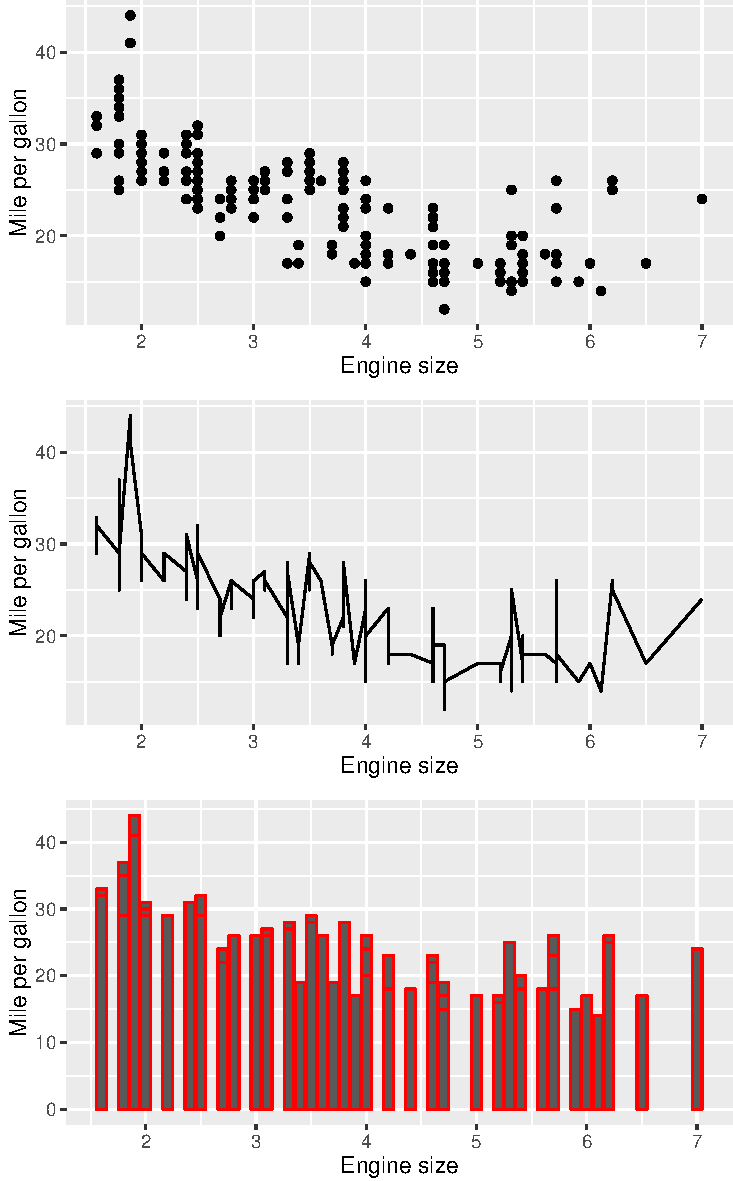
\includegraphics[width=\maxwidth]{figure/unnamed-chunk-8-1} 

\end{knitrout}

\begin{knitrout}
\definecolor{shadecolor}{rgb}{0.969, 0.969, 0.969}\color{fgcolor}\begin{kframe}
\begin{alltt}
\hlcom{### d}

\hlkwd{library}\hlstd{(lme4)}

\hlstd{lm_fdi_me} \hlkwb{=} \hlkwd{lmer}\hlstd{(fdignp} \hlopt{~} \hlstd{lag1_newtar} \hlopt{+} \hlstd{l1gdp_pc} \hlopt{+} \hlstd{l1polity} \hlopt{+} \hlstd{date} \hlopt{+} \hlstd{(}\hlnum{1} \hlopt{+} \hlstd{lag1_newtar} \hlopt{|}
    \hlstd{ctylabel),} \hlkwc{data} \hlstd{= LDC)}
\end{alltt}


{\ttfamily\noindent\color{warningcolor}{\#\# Warning: Some predictor variables are on very different scales: consider rescaling}}\begin{alltt}
\hlkwd{summary}\hlstd{(lm_fdi_me)}
\end{alltt}
\begin{verbatim}
## Linear mixed model fit by REML ['lmerMod']
## Formula: 
## fdignp ~ lag1_newtar + l1gdp_pc + l1polity + date + (1 + lag1_newtar |  
##     ctylabel)
##    Data: LDC
## 
## REML criterion at convergence: 2899.1
## 
## Scaled residuals: 
##     Min      1Q  Median      3Q     Max 
## -5.3694 -0.4273 -0.0948  0.2668  5.2309 
## 
## Random effects:
##  Groups   Name        Variance  Std.Dev. Corr 
##  ctylabel (Intercept) 12.992466 3.60451       
##           lag1_newtar  0.008787 0.09374  -0.97
##  Residual              2.783550 1.66840       
## Number of obs: 683, groups:  ctylabel, 92
## 
## Fixed effects:
##               Estimate Std. Error t value
## (Intercept) -3.341e+02  3.719e+01  -8.983
## lag1_newtar -1.900e-02  1.416e-02  -1.342
## l1gdp_pc     6.643e-05  1.012e-04   0.656
## l1polity    -4.312e-03  1.782e-02  -0.242
## date         1.687e-01  1.861e-02   9.067
## 
## Correlation of Fixed Effects:
##             (Intr) lg1_nw l1gdp_ l1plty
## lag1_newtar -0.342                     
## l1gdp_pc    -0.050  0.097              
## l1polity     0.396 -0.034 -0.225       
## date        -1.000  0.331  0.045 -0.396
## fit warnings:
## Some predictor variables are on very different scales: consider rescaling
\end{verbatim}
\end{kframe}
\end{knitrout}

Interpretation: In the random-coefficients model estimated above, we assume that both the intercept and the coefficient of newtar are normally distributed across our units. This method allows us to capture differences in the effect that tariff levels may have on FDI changes for different countries. Both the regression output and the graph below show us that in the majority of cases the effect of tariff levels is not statistically significant from zero. With a t-value of -1.342, the coefficient is not statistically significant at common levels of significance.

\begin{knitrout}
\definecolor{shadecolor}{rgb}{0.969, 0.969, 0.969}\color{fgcolor}\begin{kframe}
\begin{alltt}
\hlstd{dist2} \hlkwb{=} \hlkwd{coef}\hlstd{(lm_fdi_me)}\hlopt{$}\hlstd{ctylabel}

\hlkwd{plot}\hlstd{(}\hlkwd{density}\hlstd{(dist2}\hlopt{$}\hlstd{lag1_newtar))}
\end{alltt}
\end{kframe}
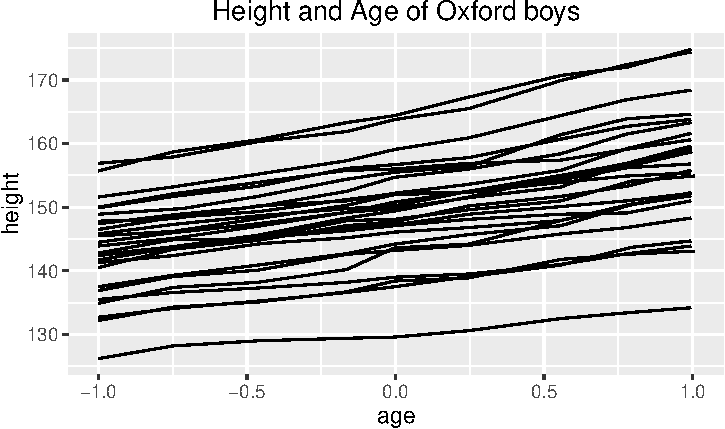
\includegraphics[width=\maxwidth]{figure/unnamed-chunk-10-1} 

\end{knitrout}



\subsection*{Problem 3}

\begin{knitrout}
\definecolor{shadecolor}{rgb}{0.969, 0.969, 0.969}\color{fgcolor}\begin{kframe}
\begin{alltt}
\hlkwd{library}\hlstd{(rddtools)}
\end{alltt}


{\ttfamily\noindent\itshape\color{messagecolor}{\#\# Loading required package: AER\\\#\# Loading required package: car\\\#\# Loading required package: lmtest\\\#\# Loading required package: zoo\\\#\# \\\#\# Attaching package: 'zoo'\\\#\# \\\#\# The following objects are masked from 'package:base':\\\#\# \\\#\#\ \ \ \  as.Date, as.Date.numeric\\\#\# \\\#\# Loading required package: sandwich\\\#\# Loading required package: survival\\\#\# Loading required package: np\\\#\# Nonparametric Kernel Methods for Mixed Datatypes (version 0.60-2)\\\#\# [vignette("{}np\_faq"{},package="{}np"{}) provides answers to frequently asked questions]}}\begin{alltt}
\hlkwd{setwd}\hlstd{(}\hlstr{"C:/Users/Jan/OneDrive/Documents/GitHub/ps630_lab/w13/"}\hlstd{)}
\hlkwd{load}\hlstd{(}\hlstr{"SocialSecurity.Rdata"}\hlstd{)}
\hlkwd{summary}\hlstd{(SocialSecurity)}
\end{alltt}
\begin{verbatim}
##  LibPartyVoteShare SocialSecurityExp
##  Min.   :15.02     Min.   :128.6    
##  1st Qu.:42.84     1st Qu.:206.9    
##  Median :49.35     Median :229.8    
##  Mean   :49.36     Mean   :233.5    
##  3rd Qu.:56.18     3rd Qu.:261.2    
##  Max.   :82.87     Max.   :323.5
\end{verbatim}
\begin{alltt}
\hlstd{social_rdd} \hlkwb{<-} \hlkwd{rdd_data}\hlstd{(}\hlkwc{y} \hlstd{= SocialSecurity}\hlopt{$}\hlstd{SocialSecurityExp,} \hlkwc{x} \hlstd{= SocialSecurity}\hlopt{$}\hlstd{LibPartyVoteShare,}
    \hlkwc{cutpoint} \hlstd{=} \hlnum{50}\hlstd{)}

\hlkwd{summary}\hlstd{(social_rdd)}
\end{alltt}
\begin{verbatim}
## ### rdd_data object ###
## 
## Cutpoint: 50 
## Sample size: 
## 	-Full : 1000 
## 	-Left : 525 
## 	-Right: 475
## Covariates: no
\end{verbatim}
\begin{alltt}
\hlkwd{plot}\hlstd{(social_rdd)}
\end{alltt}
\end{kframe}
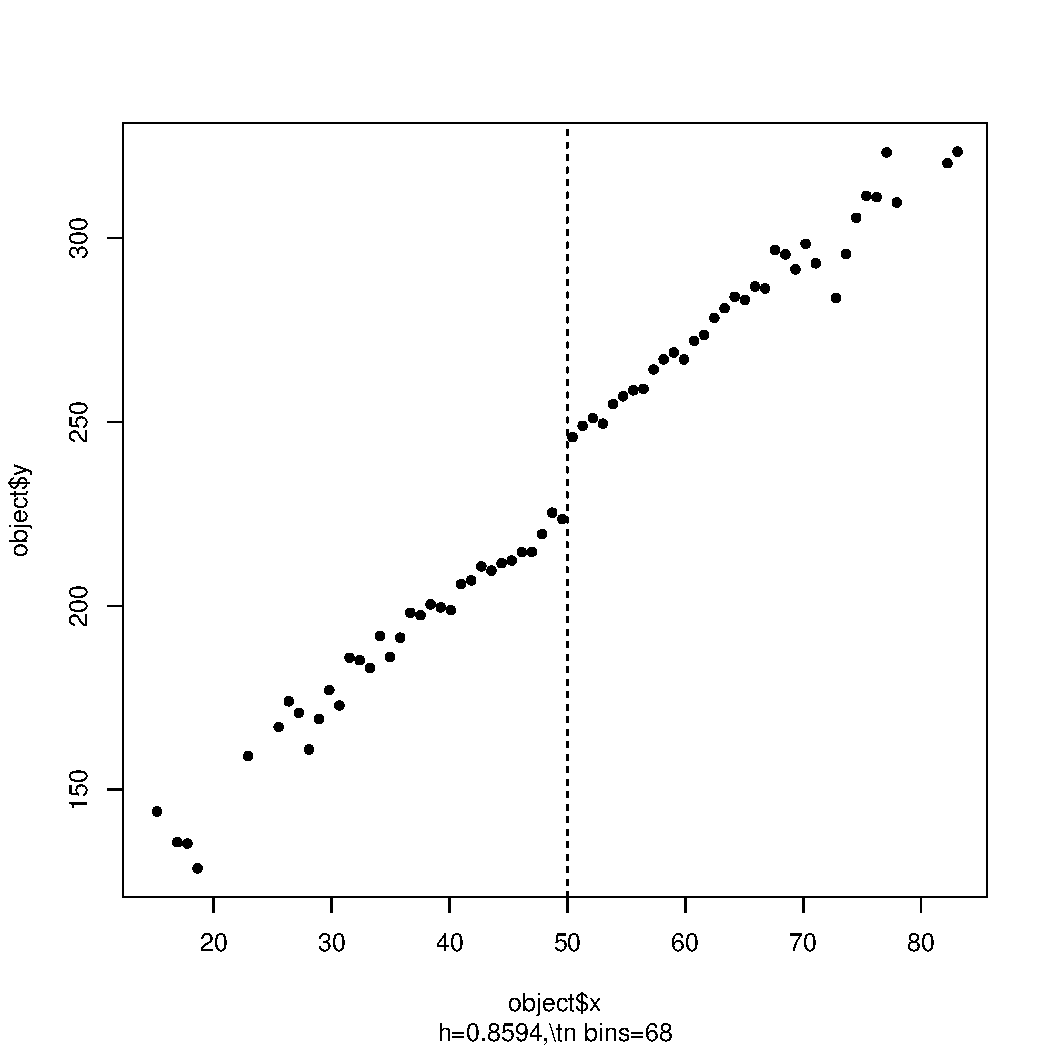
\includegraphics[width=\maxwidth]{figure/unnamed-chunk-11-1} 
\begin{kframe}\begin{alltt}
\hlstd{reg_para} \hlkwb{<-} \hlkwd{rdd_reg_lm}\hlstd{(}\hlkwc{rdd_object} \hlstd{= social_rdd,} \hlkwc{order} \hlstd{=} \hlnum{1}\hlstd{,} \hlkwc{bw} \hlstd{=} \hlnum{15}\hlstd{)}
\hlstd{reg_para}
\end{alltt}
\begin{verbatim}
## ### RDD regression: parametric ###
## 	Polynomial order:  1 
## 	Slopes:  separate 
## 	Bandwidth:  15 
## 	Number of obs: 873 (left: 450, right: 423)
## 
## 	Coefficient:
##   Estimate Std. Error t value  Pr(>|t|)    
## D  20.1724     1.2643  15.955 < 2.2e-16 ***
## ---
## Signif. codes:  0 '***' 0.001 '**' 0.01 '*' 0.05 '.' 0.1 ' ' 1
\end{verbatim}
\begin{alltt}
\hlkwd{plot}\hlstd{(reg_para)}
\end{alltt}
\end{kframe}
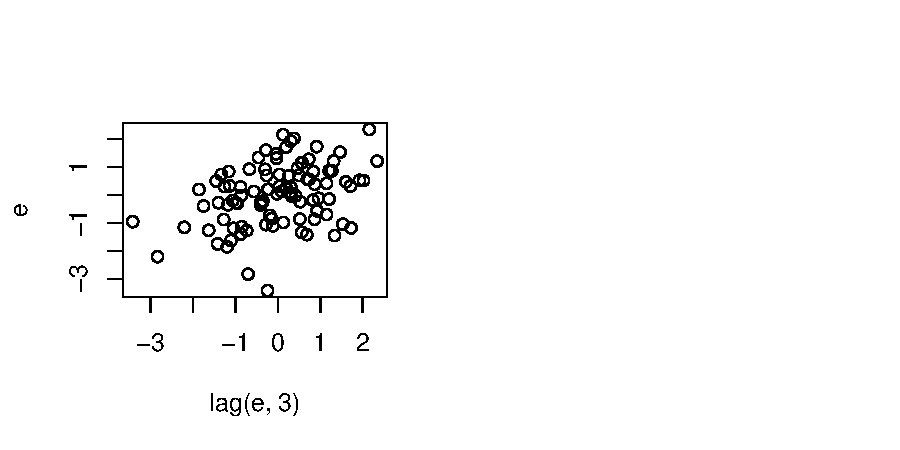
\includegraphics[width=\maxwidth]{figure/unnamed-chunk-11-2} 
\begin{kframe}\begin{alltt}
\hlstd{reg_para2} \hlkwb{<-} \hlkwd{rdd_reg_lm}\hlstd{(}\hlkwc{rdd_object} \hlstd{= social_rdd,} \hlkwc{order} \hlstd{=} \hlnum{3}\hlstd{,} \hlkwc{bw} \hlstd{=} \hlnum{15}\hlstd{)}
\hlstd{reg_para2}
\end{alltt}
\begin{verbatim}
## ### RDD regression: parametric ###
## 	Polynomial order:  3 
## 	Slopes:  separate 
## 	Bandwidth:  15 
## 	Number of obs: 873 (left: 450, right: 423)
## 
## 	Coefficient:
##   Estimate Std. Error t value  Pr(>|t|)    
## D   18.820      2.423  7.7672 2.268e-14 ***
## ---
## Signif. codes:  0 '***' 0.001 '**' 0.01 '*' 0.05 '.' 0.1 ' ' 1
\end{verbatim}
\begin{alltt}
\hlkwd{plot}\hlstd{(reg_para2)}
\end{alltt}
\end{kframe}
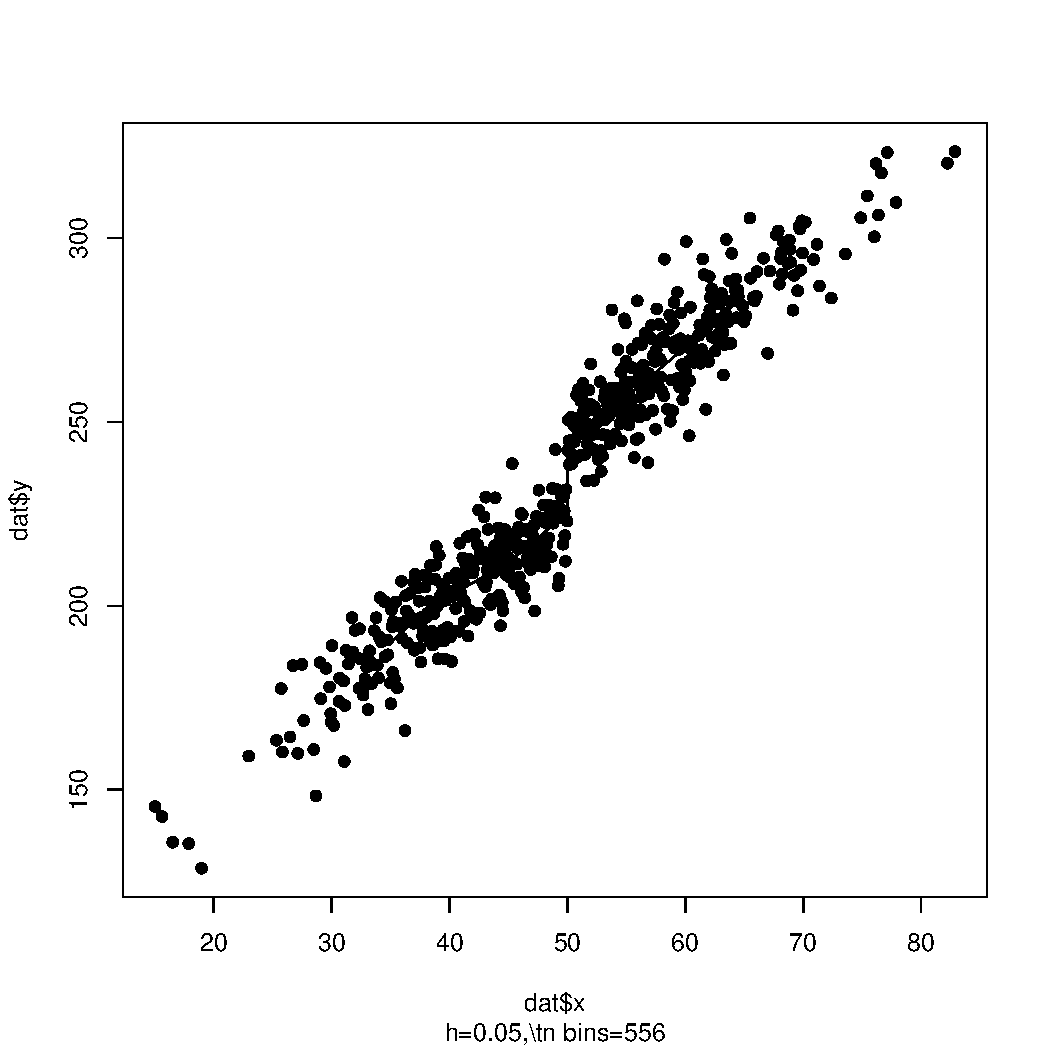
\includegraphics[width=\maxwidth]{figure/unnamed-chunk-11-3} 

\end{knitrout}

Interpretation: Both the parametric regression of first order and the third order show a very similar result. With a p-value of $p < 0.001$, the positive effect of liberal-party victories on social security expenditures is statistically significant at all common levels of significance. The magnitude of the effect appears to be very close to the value 20. This result holds for both models, increasing our confidence in its validity.

\begin{knitrout}
\definecolor{shadecolor}{rgb}{0.969, 0.969, 0.969}\color{fgcolor}\begin{kframe}
\begin{alltt}
\hlstd{bw_ik} \hlkwb{<-} \hlkwd{rdd_bw_ik}\hlstd{(social_rdd)}
\hlstd{reg_nonpara} \hlkwb{<-} \hlkwd{rdd_reg_np}\hlstd{(}\hlkwc{rdd_object} \hlstd{= social_rdd,} \hlkwc{bw} \hlstd{= bw_ik)}
\hlkwd{summary}\hlstd{(reg_nonpara)}
\end{alltt}
\begin{verbatim}
## ### RDD regression: nonparametric local linear###
## 	Bandwidth:  19.17948 
## 	Number of obs: 948 (left: 498, right: 450)
## 
## 	Weighted Residuals:
##      Min       1Q   Median       3Q      Max 
## -27.6812  -6.9454  -0.0852   6.9433  30.4306 
## 
## 	Coefficient:
##   Estimate Std. Error z value  Pr(>|z|)    
## D   20.100      2.232  9.0056 < 2.2e-16 ***
## ---
## Signif. codes:  0 '***' 0.001 '**' 0.01 '*' 0.05 '.' 0.1 ' ' 1
## 
## 	Local R squared: 0.8492
\end{verbatim}
\begin{alltt}
\hlkwd{print}\hlstd{(reg_nonpara)}
\end{alltt}
\begin{verbatim}
## ### RDD regression: nonparametric local linear###
## 	Bandwidth:  19.17948 
## 	Number of obs: 948 (left: 498, right: 450)
## 
## 	Coefficient:
##   Estimate Std. Error z value  Pr(>|z|)    
## D   20.100      2.232  9.0056 < 2.2e-16 ***
## ---
## Signif. codes:  0 '***' 0.001 '**' 0.01 '*' 0.05 '.' 0.1 ' ' 1
\end{verbatim}
\begin{alltt}
\hlkwd{plot}\hlstd{(reg_nonpara)}
\end{alltt}
\end{kframe}
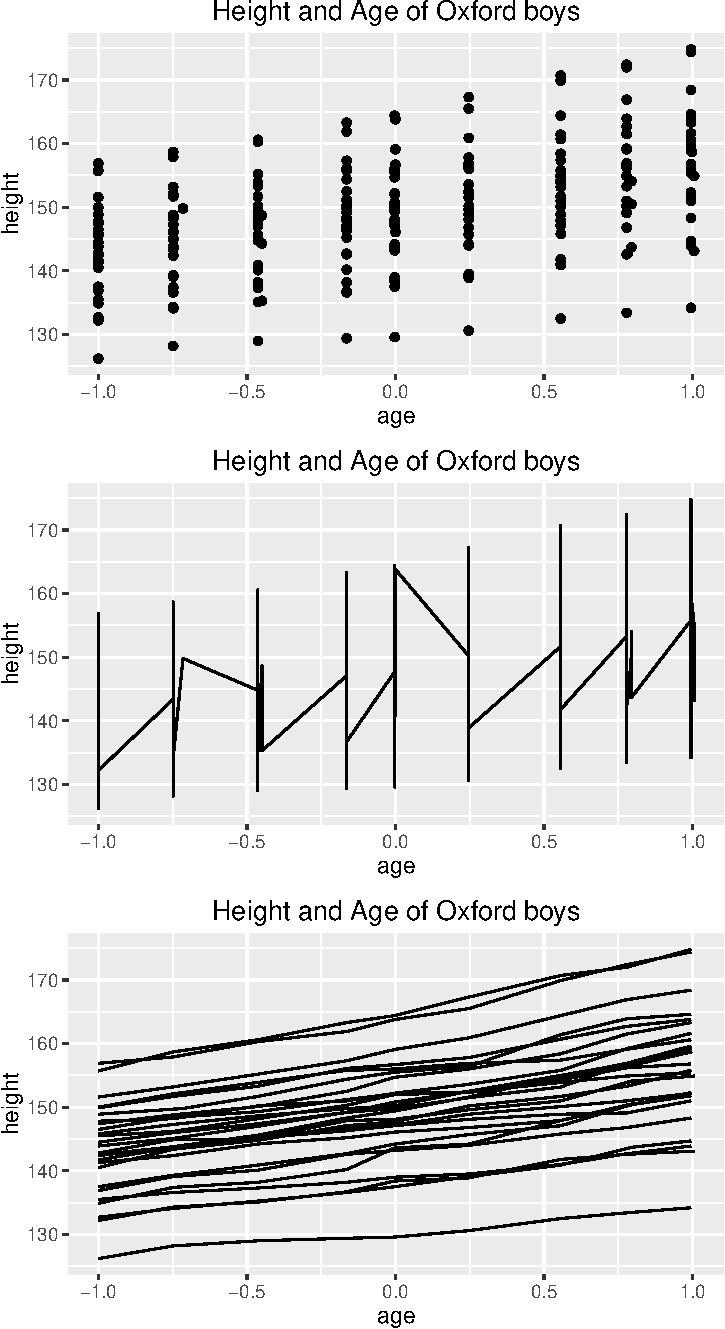
\includegraphics[width=\maxwidth]{figure/unnamed-chunk-12-1} 

\end{knitrout}

Interpretation: The nonparametric regression based on the IK optimal bandwidth confirms the result of the parametric regression. The magnitude of the estimate is once again close to the value 20 and the p-value of $p < 0.001$ indicates that this result is statistically significant at all common levels of significance.

\begin{knitrout}
\definecolor{shadecolor}{rgb}{0.969, 0.969, 0.969}\color{fgcolor}\begin{kframe}
\begin{alltt}
\hlkwd{plot}\hlstd{(reg_nonpara)}
\end{alltt}
\end{kframe}
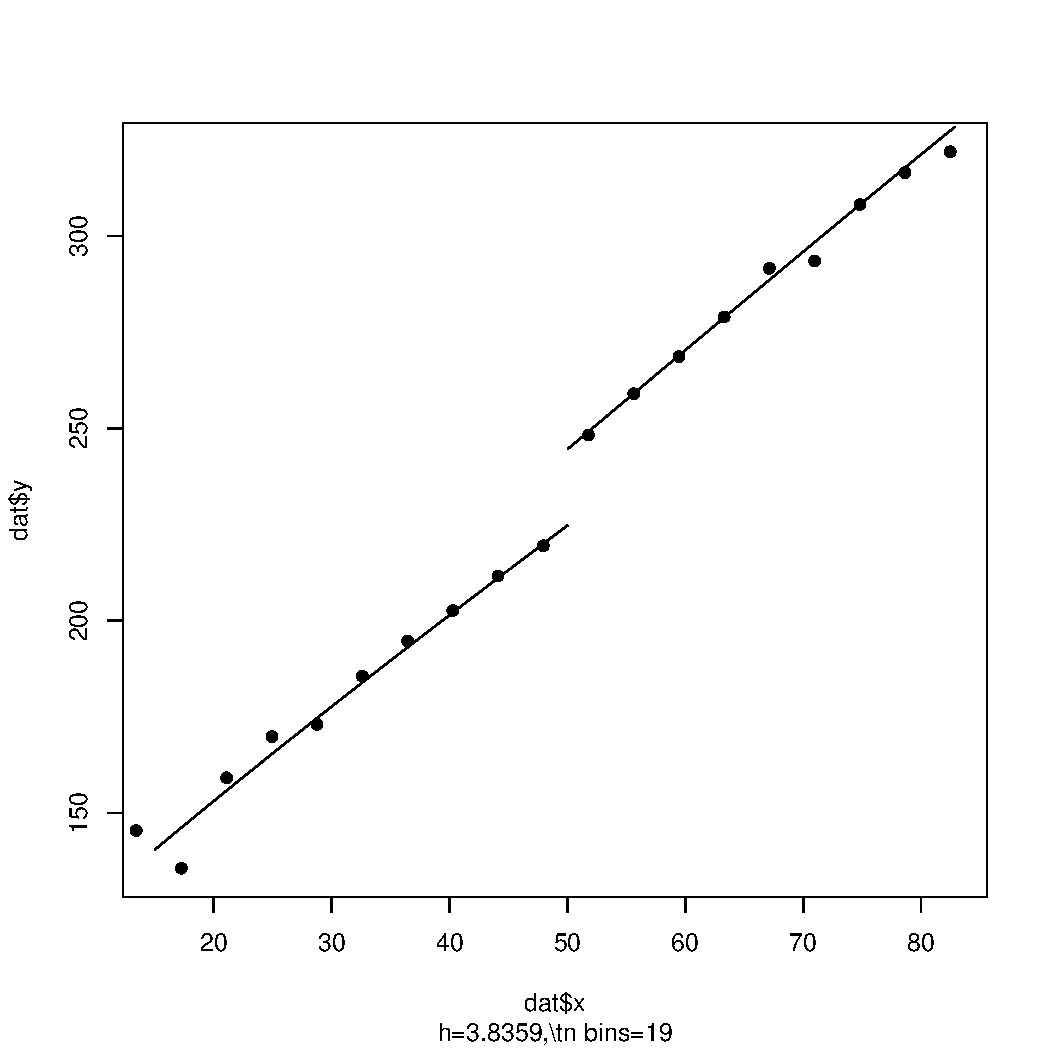
\includegraphics[width=\maxwidth]{figure/unnamed-chunk-13-1} 
\begin{kframe}\begin{alltt}
\hlkwd{plotSensi}\hlstd{(reg_nonpara,} \hlkwc{from} \hlstd{=} \hlnum{5}\hlstd{,} \hlkwc{to} \hlstd{=} \hlnum{20}\hlstd{,} \hlkwc{by} \hlstd{=} \hlnum{1}\hlstd{)}
\end{alltt}
\end{kframe}
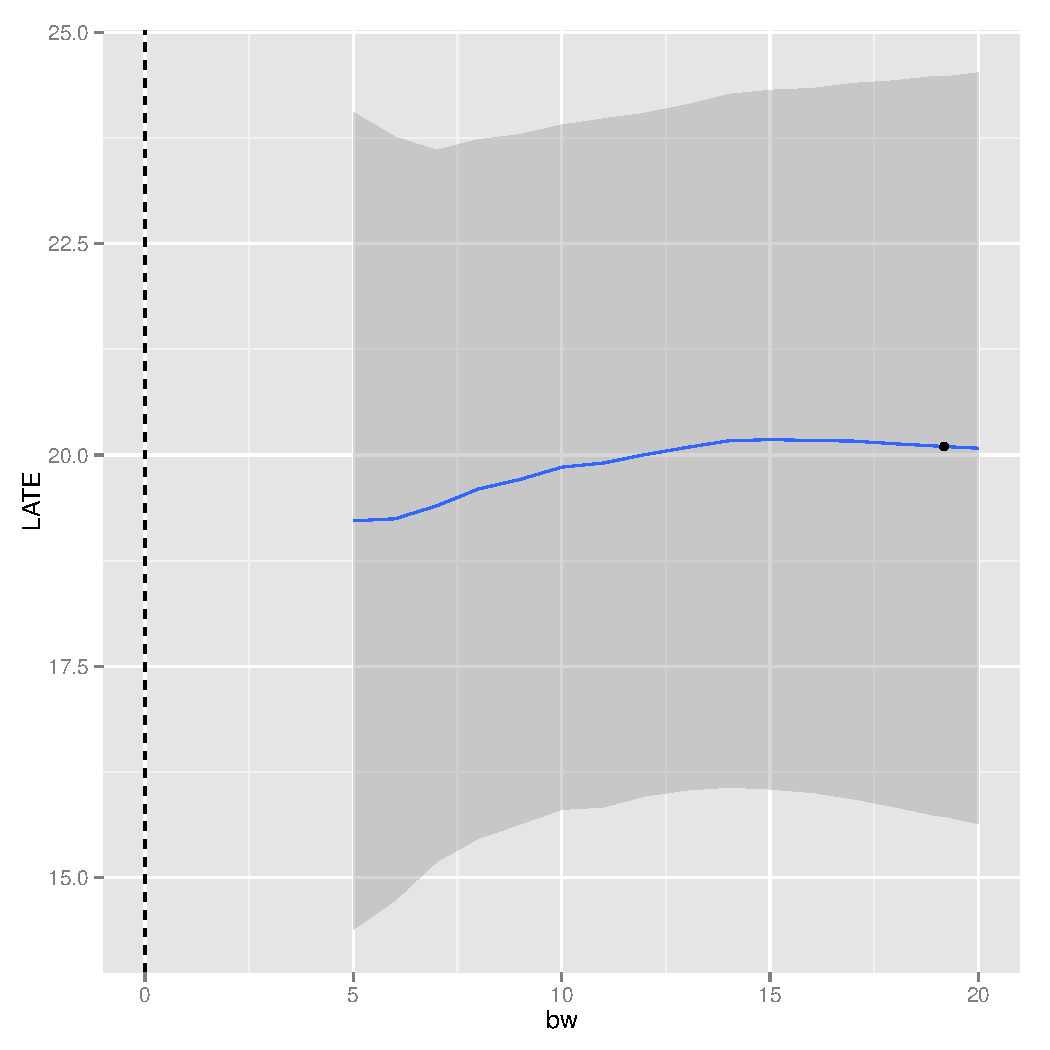
\includegraphics[width=\maxwidth]{figure/unnamed-chunk-13-2} 

\end{knitrout}

Interpretation: The sensitivity test reveals that our results are not sensitive to changes in the bandwidth. Indeed, they differ only marginally between a bandwidth of 5 and a bandwidth of 20. This should increase our confidence that the discontinuity at 50 percent is not based on arbitrary model specifications.

\begin{knitrout}
\definecolor{shadecolor}{rgb}{0.969, 0.969, 0.969}\color{fgcolor}\begin{kframe}
\begin{alltt}
\hlkwd{plotPlacebo}\hlstd{(reg_nonpara)}
\end{alltt}
\end{kframe}
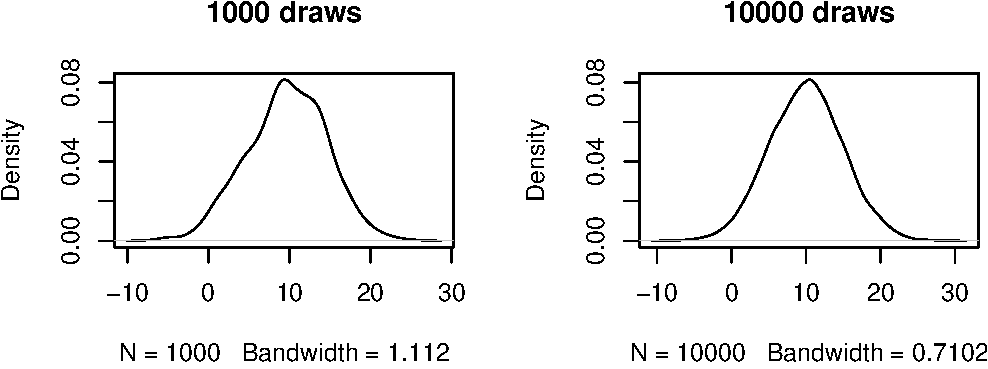
\includegraphics[width=\maxwidth]{figure/unnamed-chunk-14-1} 

\end{knitrout}

Interpretation: The Placebo test shows that, if we choose other cut-off points at random, we do not get a result that is statistically significant from zero. Indeed, it appears that all confidence intervals at other values include the value zero, meaning that we would not find any effect if we set the cut-off point at this value.

\begin{knitrout}
\definecolor{shadecolor}{rgb}{0.969, 0.969, 0.969}\color{fgcolor}\begin{kframe}
\begin{alltt}
\hlkwd{dens_test}\hlstd{(reg_nonpara)}
\end{alltt}
\end{kframe}
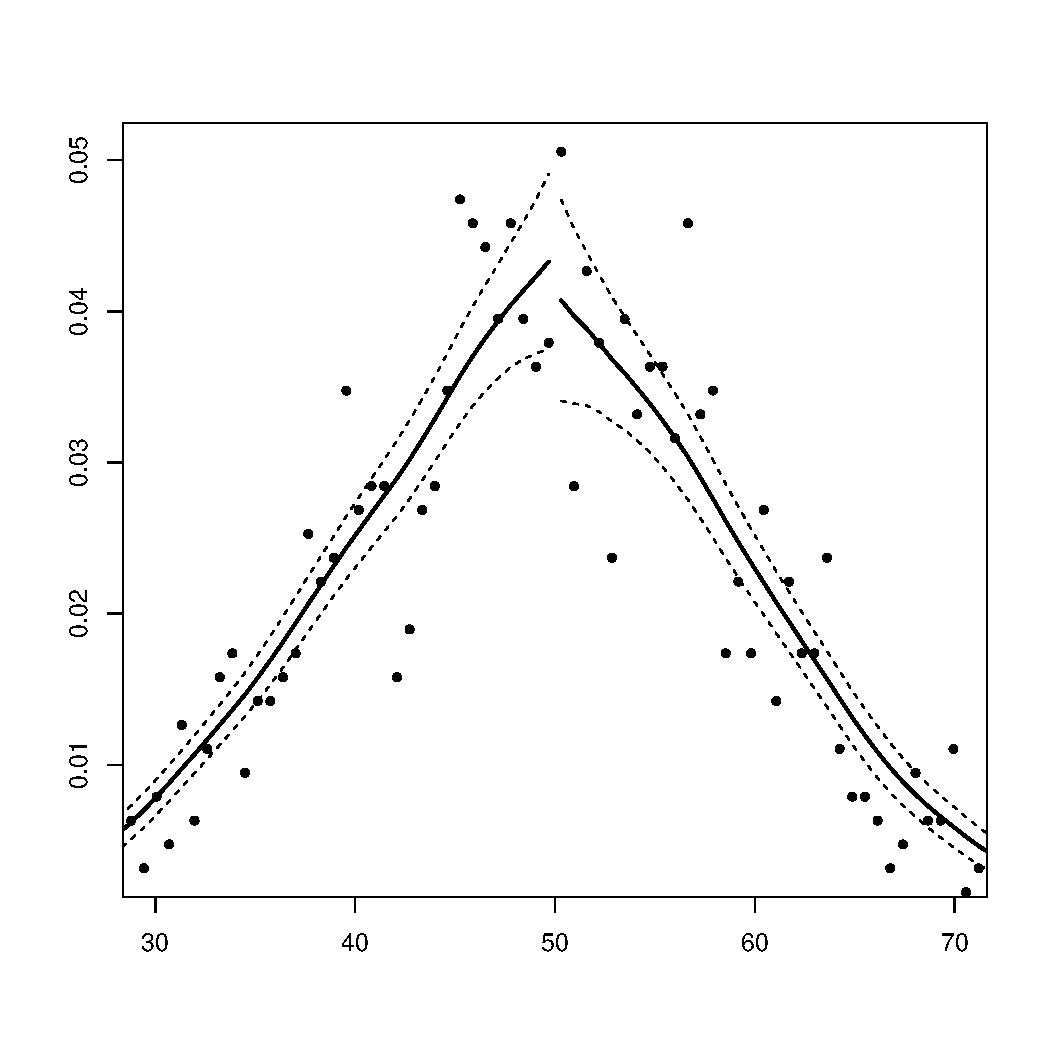
\includegraphics[width=\maxwidth]{figure/unnamed-chunk-15-1} 
\begin{kframe}\begin{verbatim}
## 
## 	McCrary Test for no discontinuity of density around cutpoint
## 
## data:  reg_nonpara
## z-val = -0.46603, p-value = 0.6412
## alternative hypothesis: Density is discontinuous around cutpoint
## sample estimates:
## Discontinuity 
##    -0.0664955
\end{verbatim}
\end{kframe}
\end{knitrout}

Interpretation: The McCrary density test fails to reject the null hypothesis that there is no discontinuity in density around the cut-off point at common levels of statistical significance. This result indicates that units are not subject to an artificial treatment. We can thus be more confident in the validity of our results.



\subsection*{Problem 4}

\subparagraph{a)} Differences-in-differences is a powerful tool for causal inference if its assumptions are true. The most crucial assumption in the simple diff-in-diff framework is the parallel trends assumption. Why is this the case? We compare the characteristics of two groups over time. In the vast majority of cases, the characteristic of interest is not static but moves. The parallel trends assumption means \textit{that the characteristic of interest does not trend for the two groups in a systematically different way}. Note that there may still be some degree of random error for individual observations but as long as we have a sufficiently large number of observations drawn at random from the population, this random error will not bias the results. The parallel trends assumption is such an important part of diff-in-diff because we \textit{approximate} (however, we do never perfectly meet the requirements of) a randomized experiment in which we have one control group and one treatment group.

Most importantly, if the parallel trends assumption is true for the population and individual deviations are caused by random error only, the group not affected by the treatment can \textit{plausibly function as (near-)counterfactual} to the group that is affected by it.

In other words, when the parallel trends assumption is true, the comparison of group differences at time t-1 and t reveals the effect of the exogeneous treatment that only affects one of the two groups because both groups are subject to the same intertemporal dynamics in all other respects. Accordingly, the following mathematical expression captures the magnitude of the difference:

$$ \delta = (\bar{x} _{t2} - \bar{y} _{t2}) - (\bar{x} _{t1} - \bar{y} _{t1}) $$

Where $x$ is the treatment group and $y$ is the control group and $t1$ and $t2$ indicate time points 1 and 2 respectively.

\subparagraph{b)} Without any additional model features or assumptions, when the parallel trends assumption is violated, the difference in differences could be caused by diverging intertemporal dynamics in the characteristic of interest. This means that the effect cannot be effectively reduced to the treatment by which only one group is affected. Because we cannot distinguish between the impact of the treatment and the impact of other unobserved factors, we can no longer make an inference about the magnitude of the treatment effect.

Note that this also means that we have to be very confident in the parallel trends assumption to make causal claims based on a simple diff-in-diff framework.

\subparagraph{c)} If we have three time points per group that we analyze, we can estimate time trends that are group-specific. As long as the time trend of the treatment group is correctly captured by at least two points in time before the treatment, we can still make claims about the effect that the treatment had. We can technically catpure such a trend through an interaction of unit dummies and time variables. Therefore, these individual time trends allow us to relax the parallel trends assumption. We merely need a stable trend in the analyzed groups.



\end{document}
